\chapter{Experimental Results}
\label{chapter6}
\section{Overview} 
This chapter outlines the outcomes of the cooperative spectrum sensing using soft and hard decision fusion schemes. The $P_{davg}$ vs $SNR$ plot is generated for both the schemes to compare their performance in a real fading scenario on a hardware test-bed. The data files generated using gnuradio are imported in MATLAB for all sensor nodes and the results are derived. As it is expected soft-fusion schemes outperform hard-fusion scheme but as we go to higher SNRs both the schemes generally converges to the same results. For LTE-R performance analysis we have the plot for K-factor variation inside a tunnel for high speed tunnel. We also generated the ber curves for all three modulation schemes proposed for LTE-R and it is evident from the plots for higher K-values we have good connectivity. As the train moves away from the LCXs slot, the K-factor goes down and bit-error rate increases. Finally, we generated the continuous ber curve to test the performance of LTE-R in a discrete timestep manner.

\section{Heterogeneous CSS Results}
In this thesis, we implemented the heterogeneous cooperative spectrum sensing (CSS) using both hard and soft data fusion schemes. We start by collecting the data across 450 MHz band for all sensor nodes in a distributed manner. The spectrum sensing data is normalized for both soft and hard data fusion schemes using the same operational parameters to compare their performance accurately. The measurements are performed using software-defined radios (SDRs) and the post processing is conducted on desktop computers. The desktop computer consists of i7 Intel processor with eight cores and 3.41 GHz clock cycle running Ubuntu 16.04. The sensor node network is implemented using RTL-SDR dongles and Ettus Research USRP N210 on GNU Radio Software platform.
These sensor nodes collect the spectral data, normalize it and then transmit it to the FC for the detection. For soft data fusion, the data is quantized in the local sensor nodes before it is transmitted to FC due to the limited bandwidth of the overhead channel. 

\subsection{Hard Decision Combining}
The Figure~\ref{hardres} shows the shows the $P_{davg}$ versus $SNR_{avg}$ for all four sensor nodes. It can be seen that OR performs the best while AND performs
the worst in a fading channel. The SN R avg was computed by taking the mean of all the SNRs for the sensor nodes. The SNR
was varied for each sensor node by varying the transmitter amplitude and gain in the gnuradio flowgraph.

\begin{figure}[ht!]
	\centering
	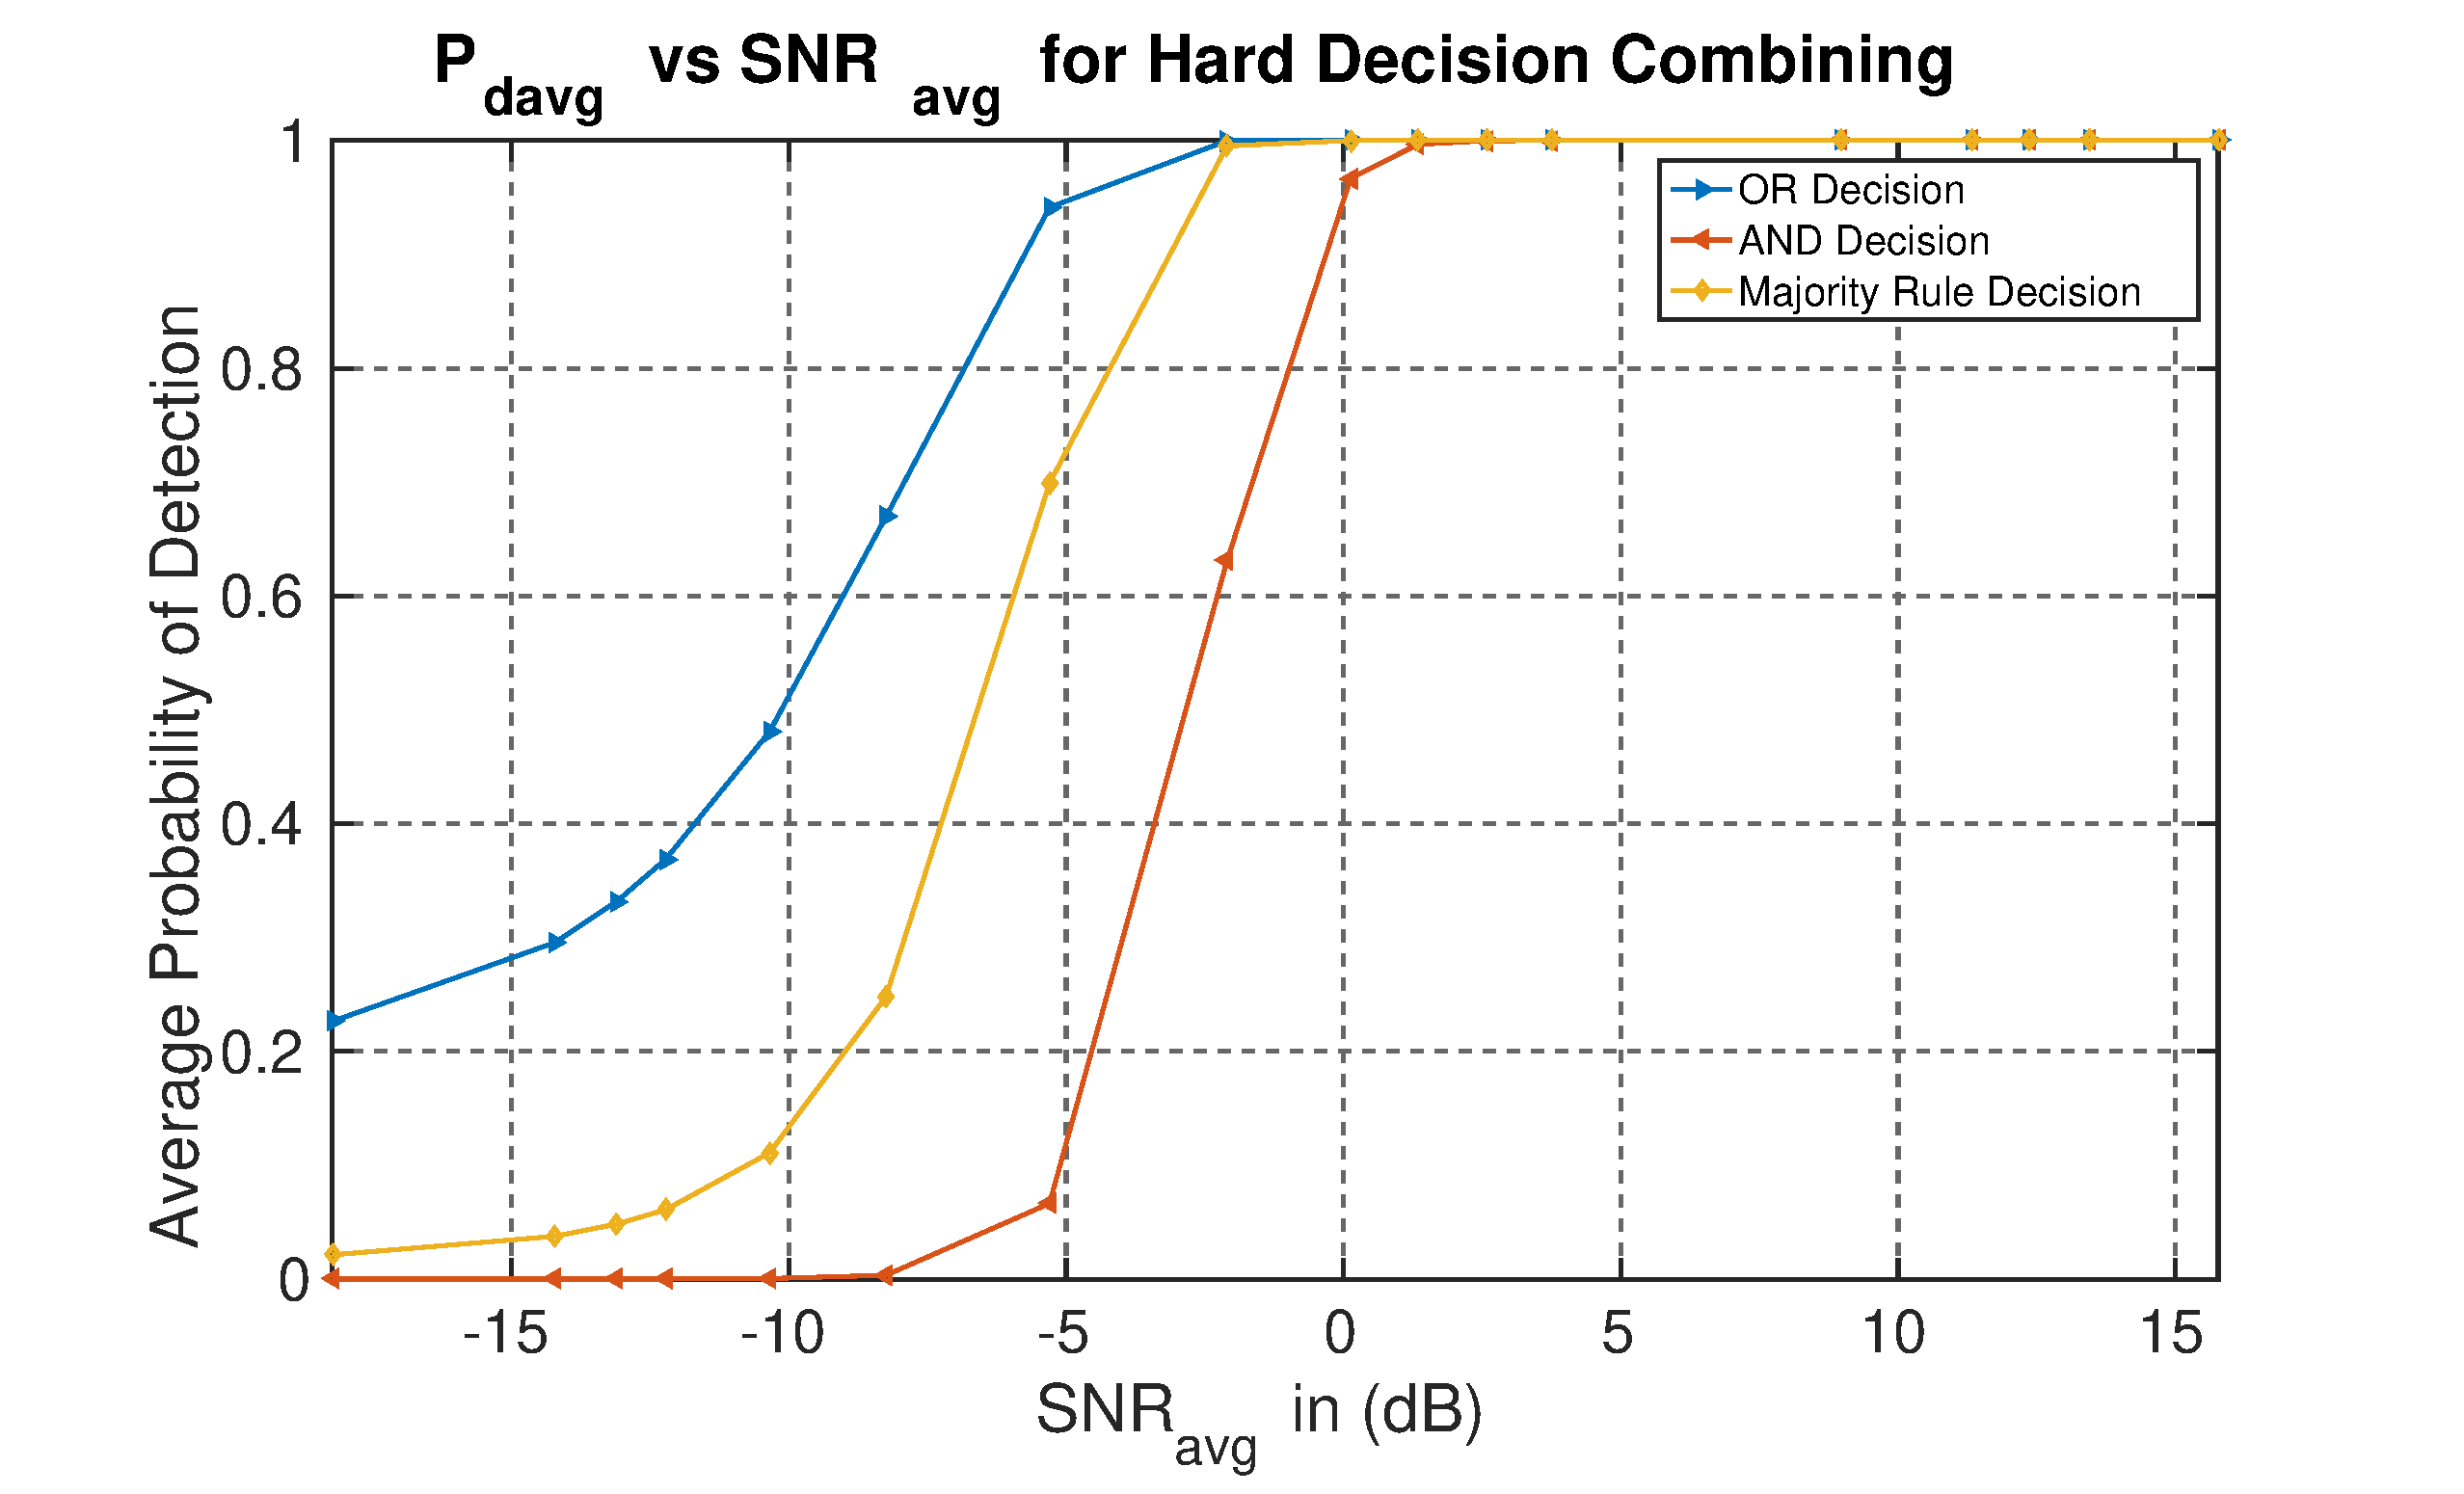
\includegraphics[width=\textwidth,keepaspectratio]{images/Gill/figs/hardecisionpd.eps}
    \caption{Probability of Detection versus $SNR_avg$ For Hard Decision Combining.} 
\label{hardres}      
\end{figure}
In Figure~\ref{hardroc} the ROC characteristics for the hard decision combining at two different $SNR_{avg}$ for all three hard data fusion schemes are provided. It is pretty evident from the plot that OR scheme performs better than both AND and majority rule scheme. The AND scheme performs the worst because it depends on all sensor nodes to have same decision which is very difficult in a real fading environment. For lower SNR values OR outperform majority rule by a large margin but as we go to higher SNR values their performance converges.

\begin{figure}[ht!]
	\centering
	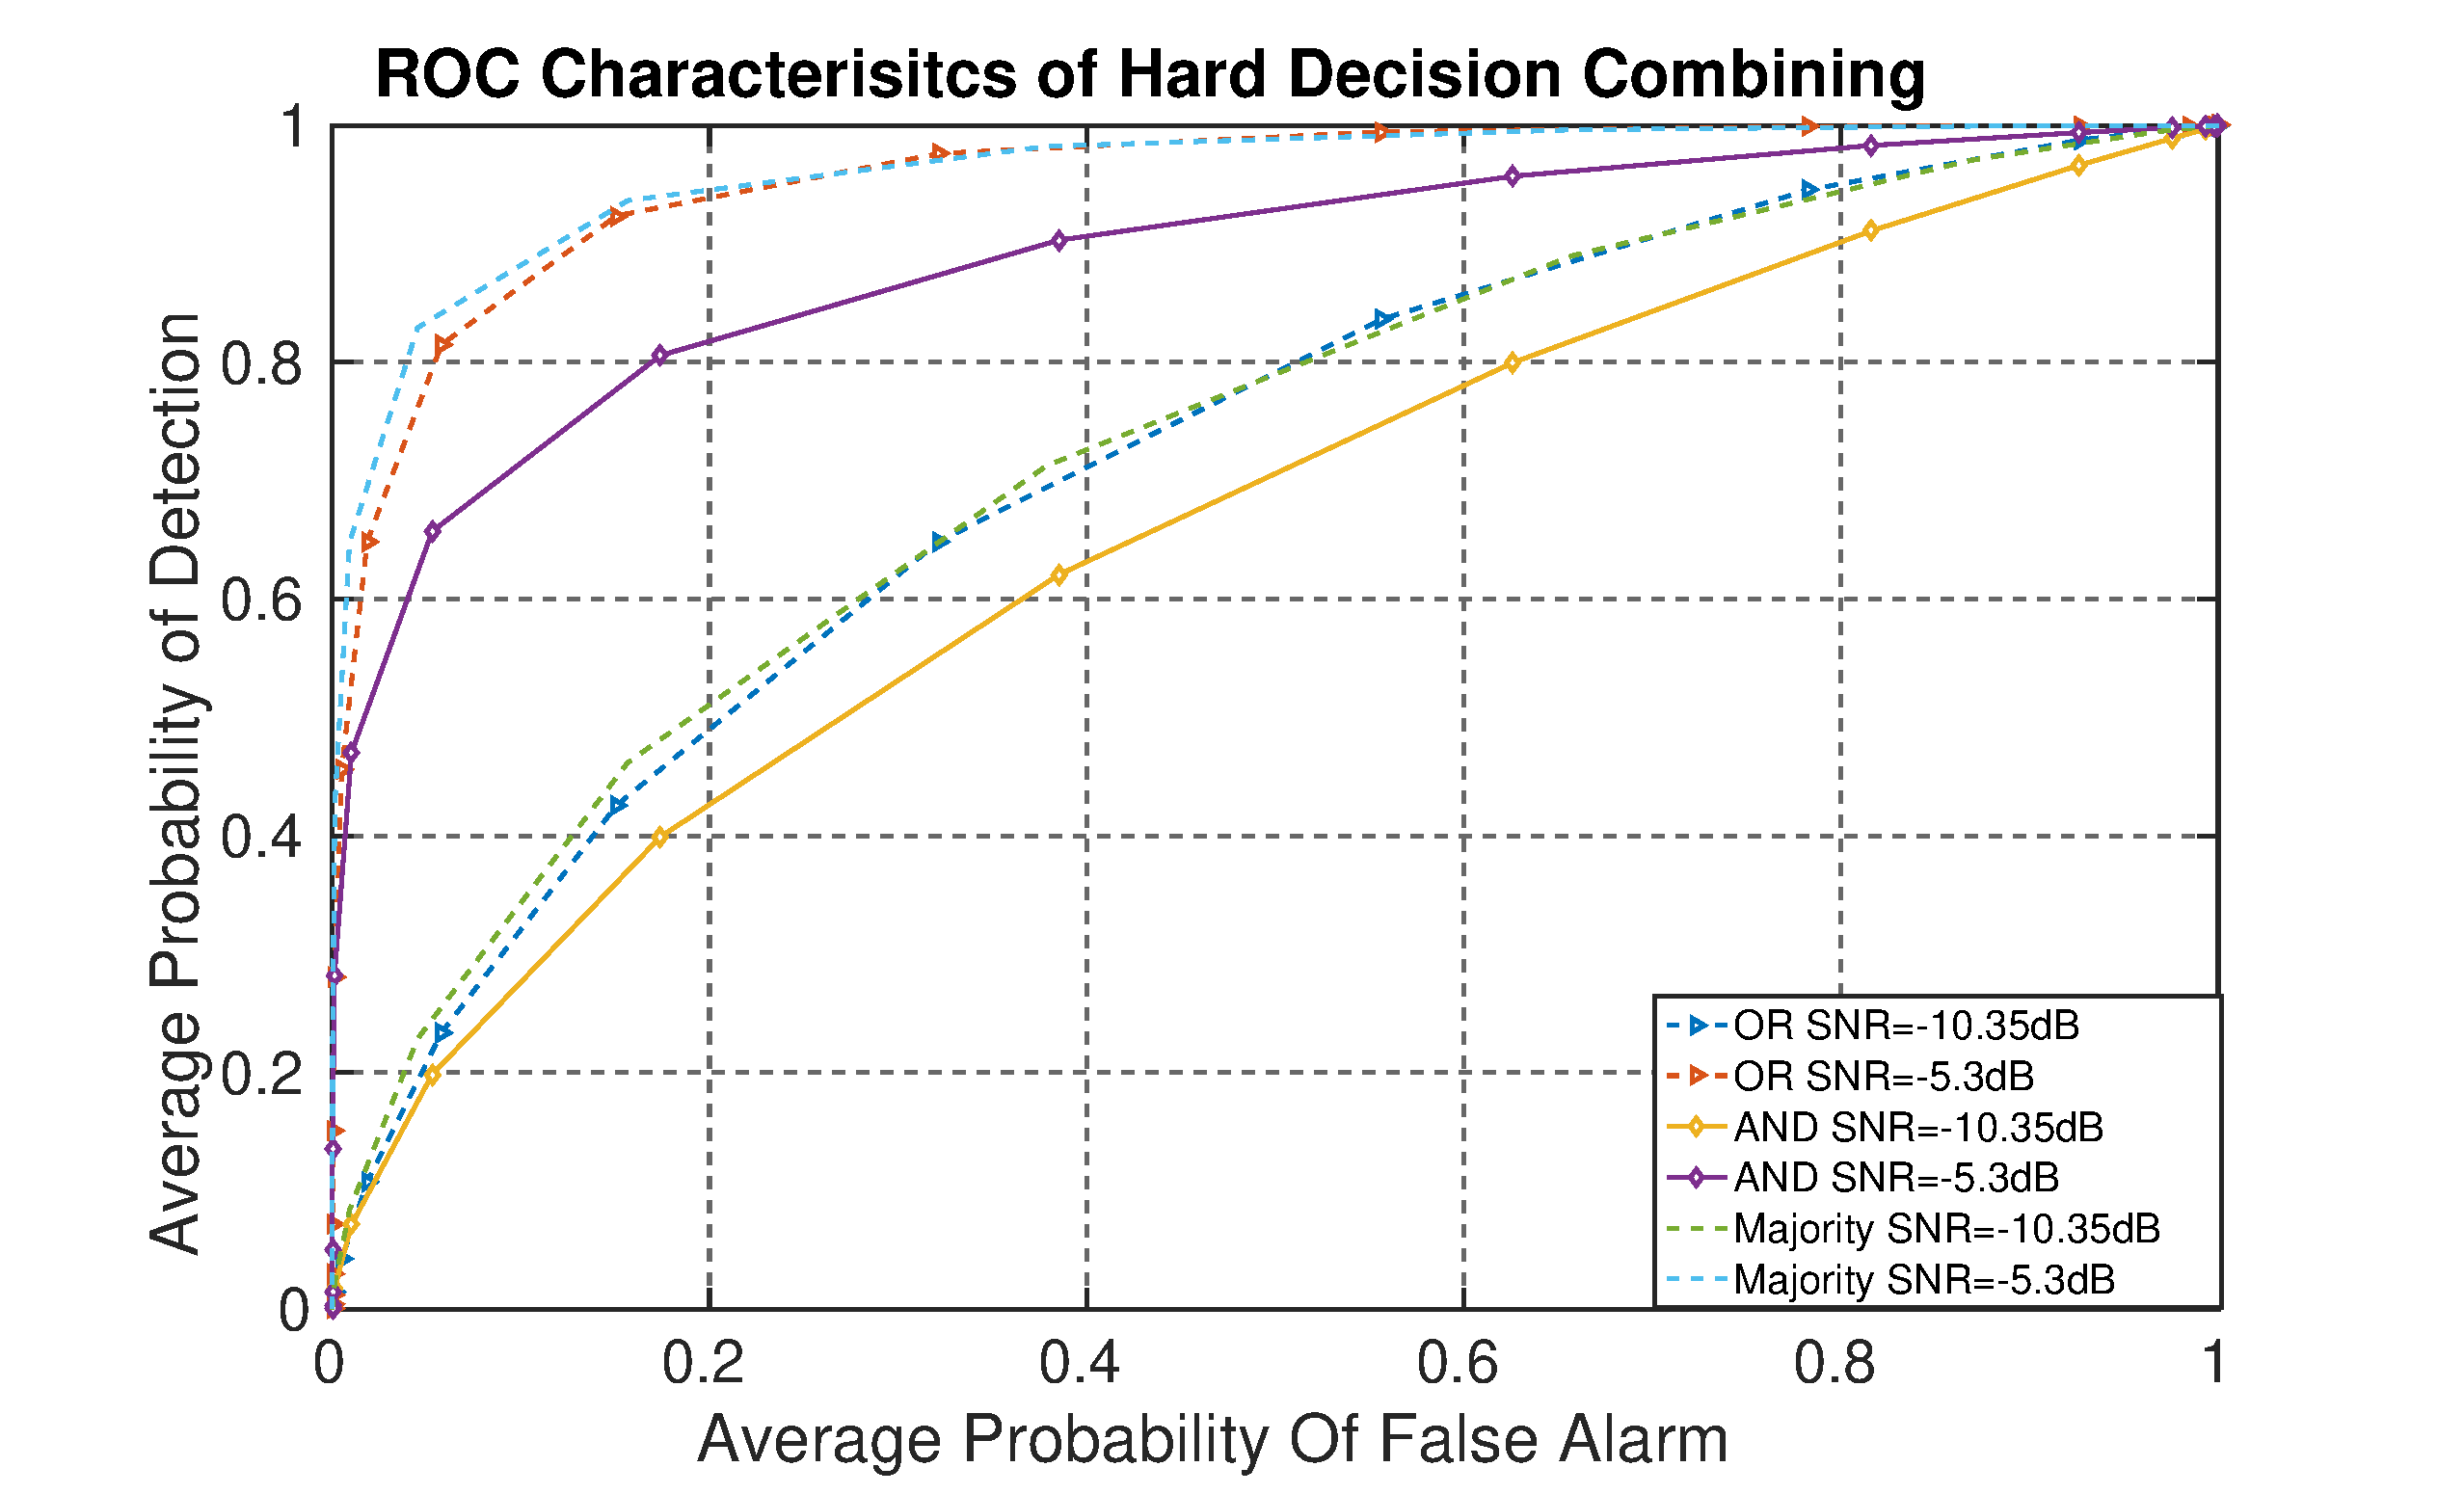
\includegraphics[width=\textwidth,keepaspectratio]{images/Gill/figs/hardecisioroc.eps}
    \caption{ROC Characteristics for Hard Decision Combining with Different SNRs.} 
\label{hardroc}      
\end{figure}

\subsection{Soft Decision Combining}
The Figure~\ref{softpd} shows the $P_{davg}$ vs $SNR_{avg}$ for both soft and hard data fusion schemes. MNE and OR scheme overlap on the plot because in MNE scheme we take the maximum normalized energy and compare it the global test statistic, whereas in OR scheme we estimate the signal source by either of sensor node decision. This makes both the scheme almost same and this is visible in the results. The EGC scheme performs the best because it takes into consideration all the sensor nodes and it's global test statistic gives equal weightage to all sensor nodes. AND scheme performs the worst as it was expected. It is very important to understand that at higher SNR values, $SNR_{avg}$ > 2 dB, we see all schemes converging to the same decisions. This tells us that in noiseless environment we can choose hard fusion schemes because of their implementation complexity and we can select soft fusion in severe fading environment as they tend to be more accurate in these scenarios.
\begin{figure}[ht!]
	\centering
	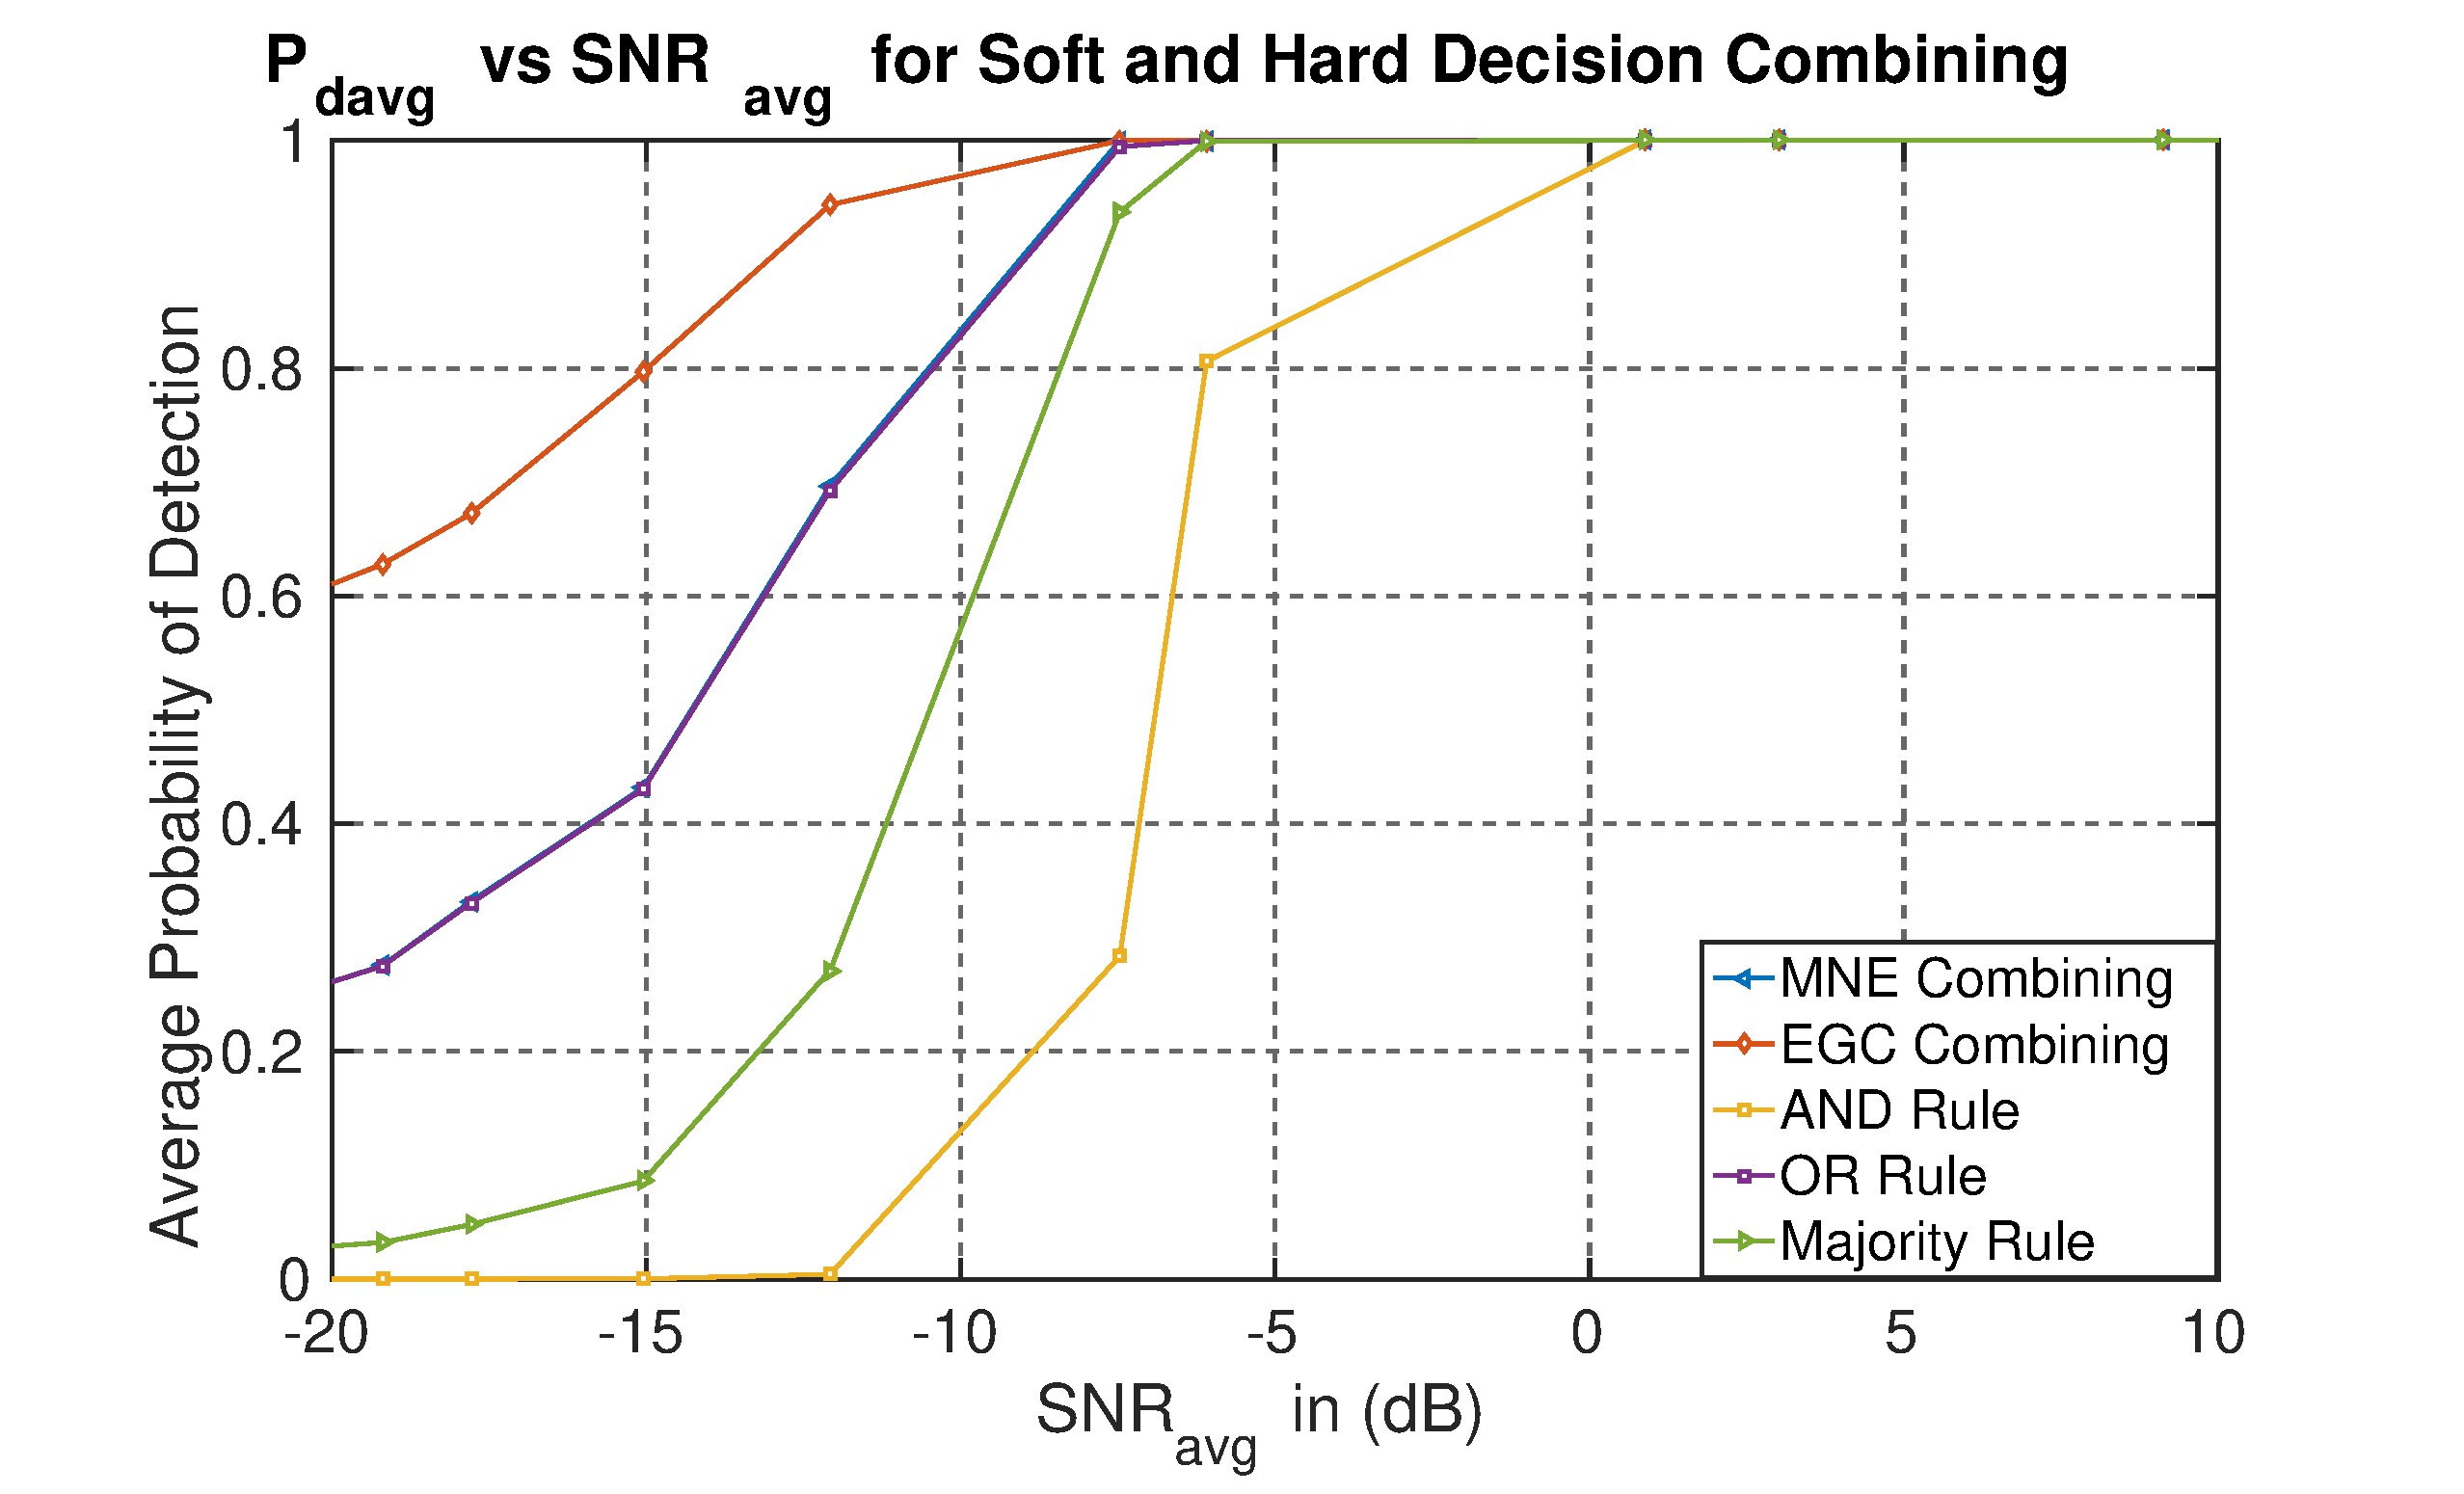
\includegraphics[width=\textwidth,keepaspectratio]{images/Gill/figs/softnhardecisionpd.eps}
    \caption{Probability of Detection versus $SNR_avg$ For Soft and Hard Decision Combining.} 
\label{softpd}      
\end{figure}




\section{HST LTE-R in a Tunnel}
Using LTE System Toolbox provided by MATLAB we generated Figure~\ref{lteofdma} which shows the received resource grid without equalization. The frame worth of data was modulated with QPSK, 16QAM and 64QAM for equal number of subcarriers and mapped to symbol in a subframe. We generate ten subframes individually and create one frame after merging all subframes. The frame is passed through our proposed high speed train channel model, with additive white gaussian noise added. We can see that without equalization the received resourced grid has lot of errrors and will lead to numerous retransmissions.

\begin{figure}[!ht]
\label{lteofdma}
\centering
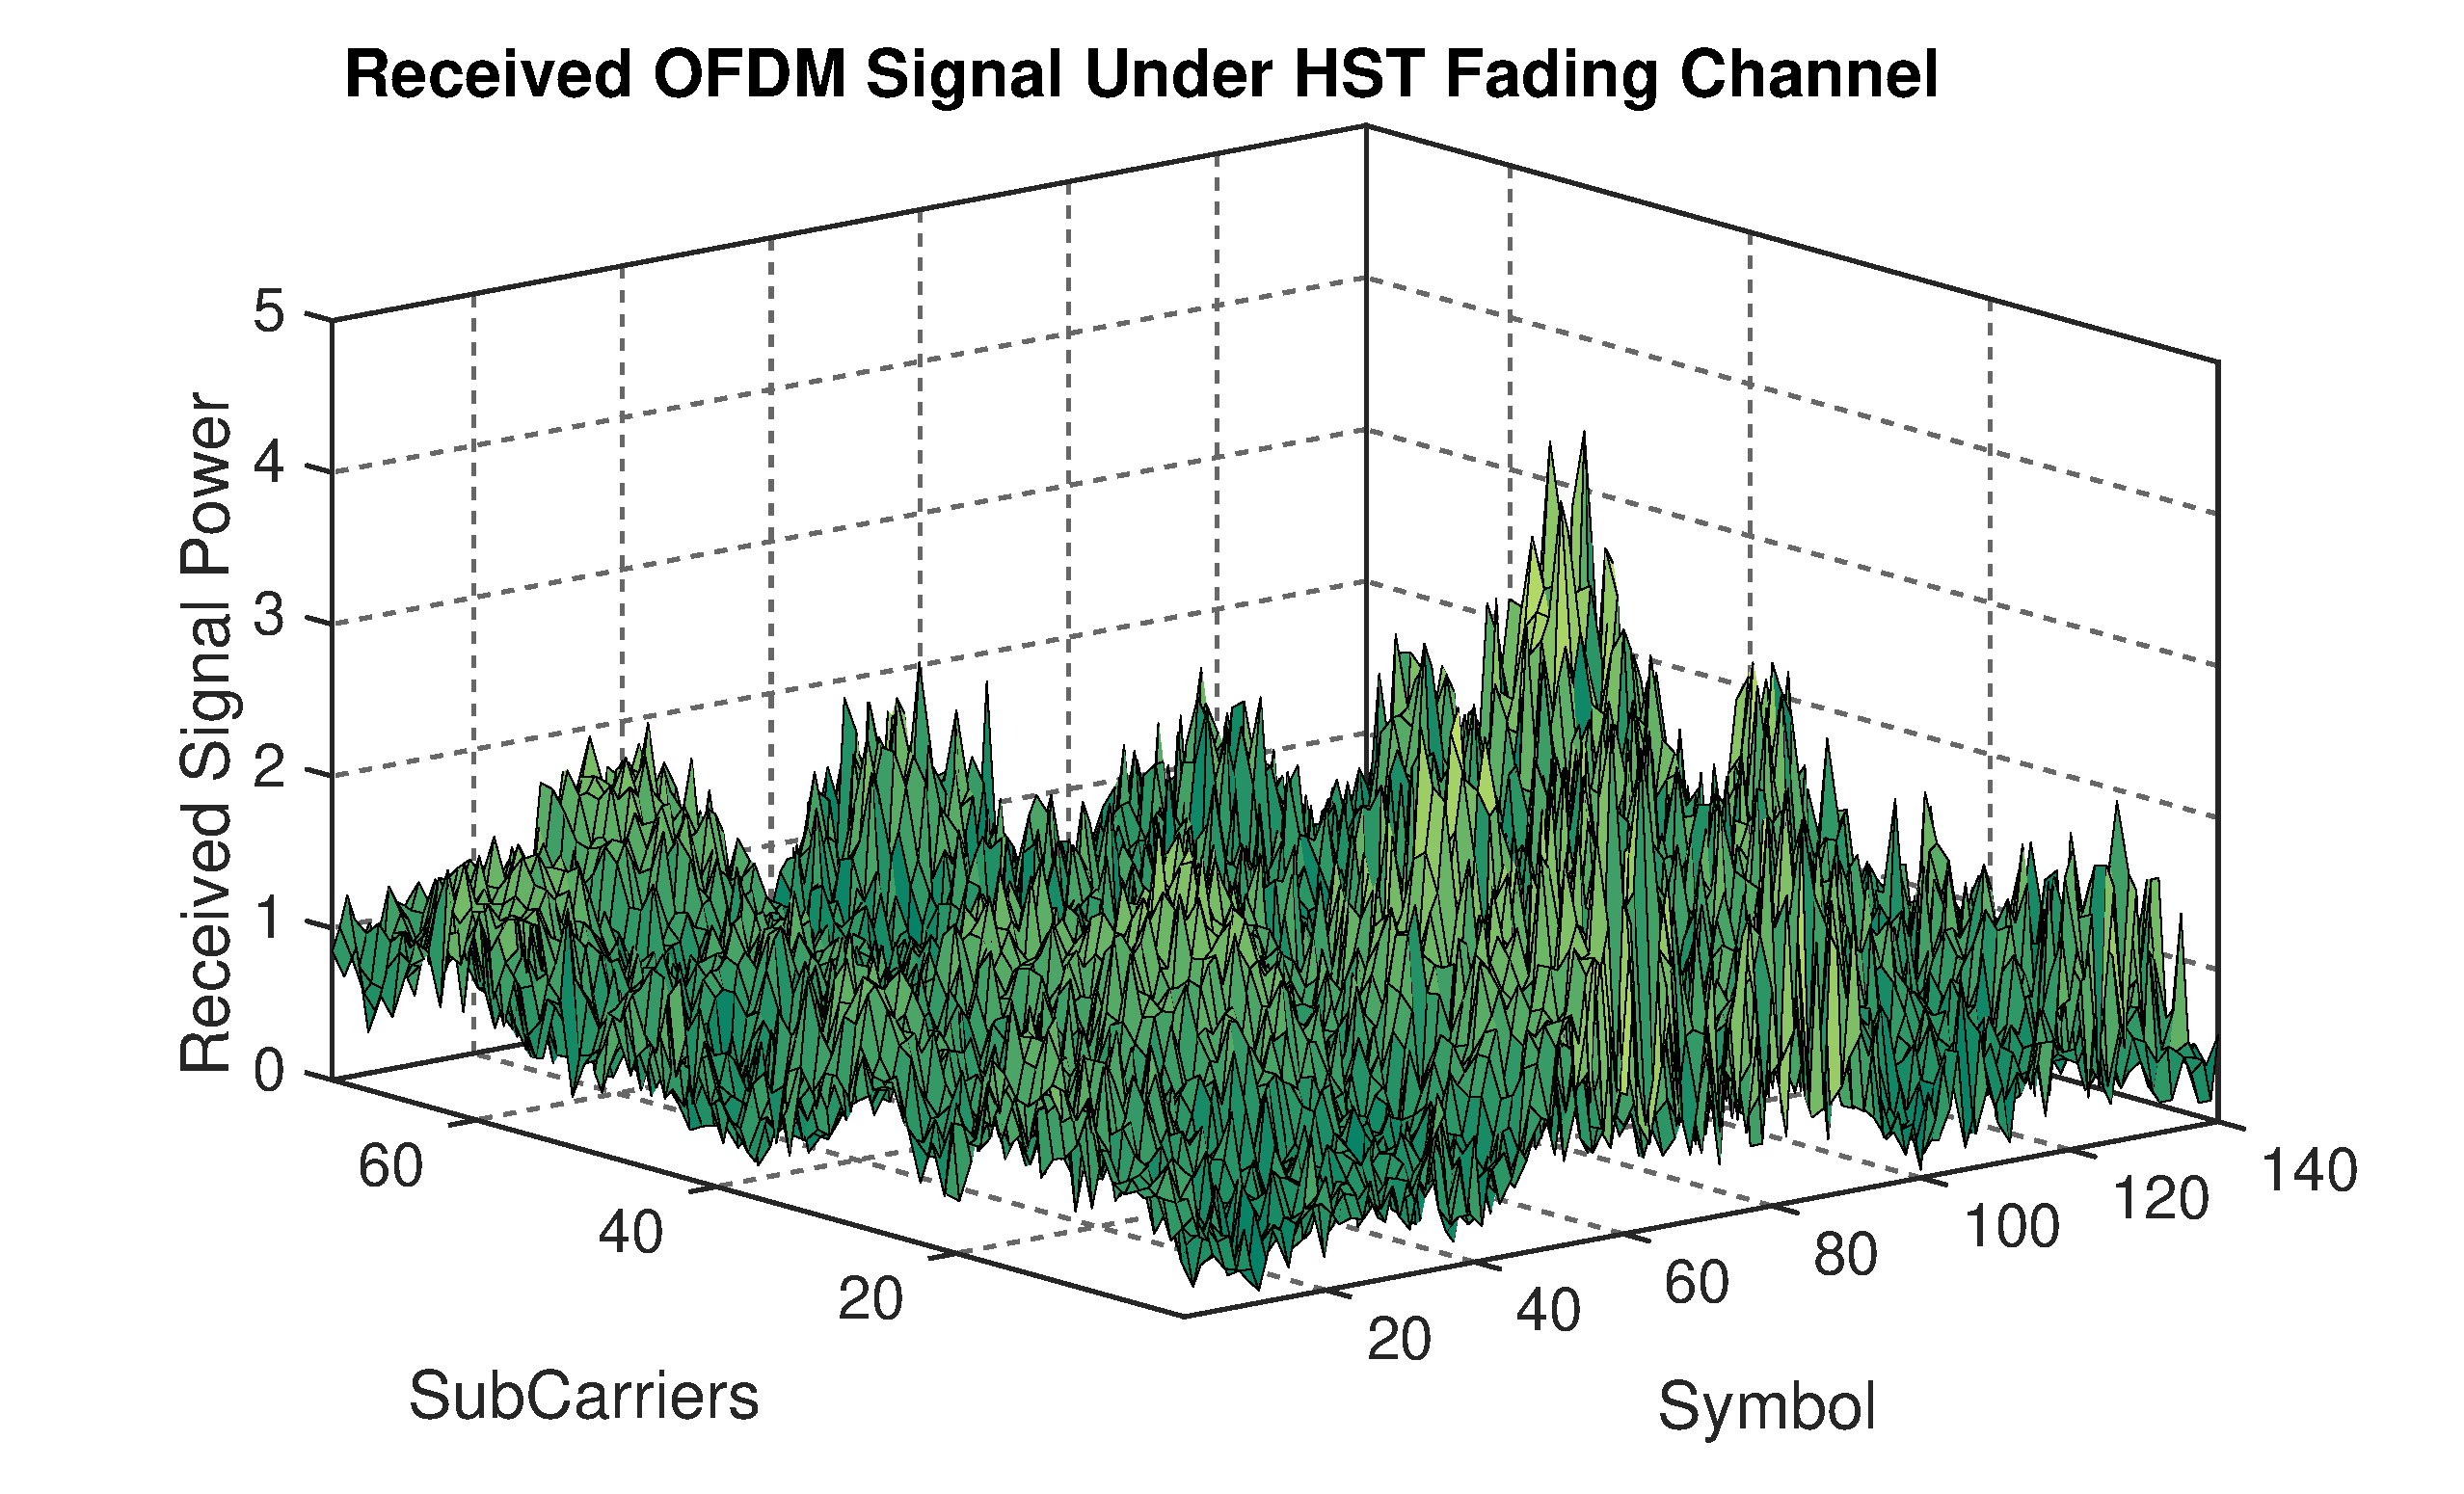
\includegraphics[width=\textwidth,keepaspectratio]{images/Gill/lte_figs/receivedsignal.eps} 
\caption{Received LTE-R OFDM signal under HST Ricean Fading Environment. }
\end{figure}

\subsection{K-factor in a Tunnel}
In Figure~\ref{kfactorber}, we calculated the K-factor for the HST inside a tunnel with velocity $v$ = 500 km/h for different center frequencies. It shows the variation of the Rician K-factor with the distance between the transmitter and receiver as the train is moving along the tunnel. We computed the K-factor for a leaky cable with periodic slots separated by distance d in fixed time-steps. The plot shows that the K-factor varies significantly over a short distances. Therefore, assuming a single K-factor for the channel model is not accurate, we use time-series K-factor to do our channel modeling.

\begin{figure}[!ht]
\label{kfactor}
\centering
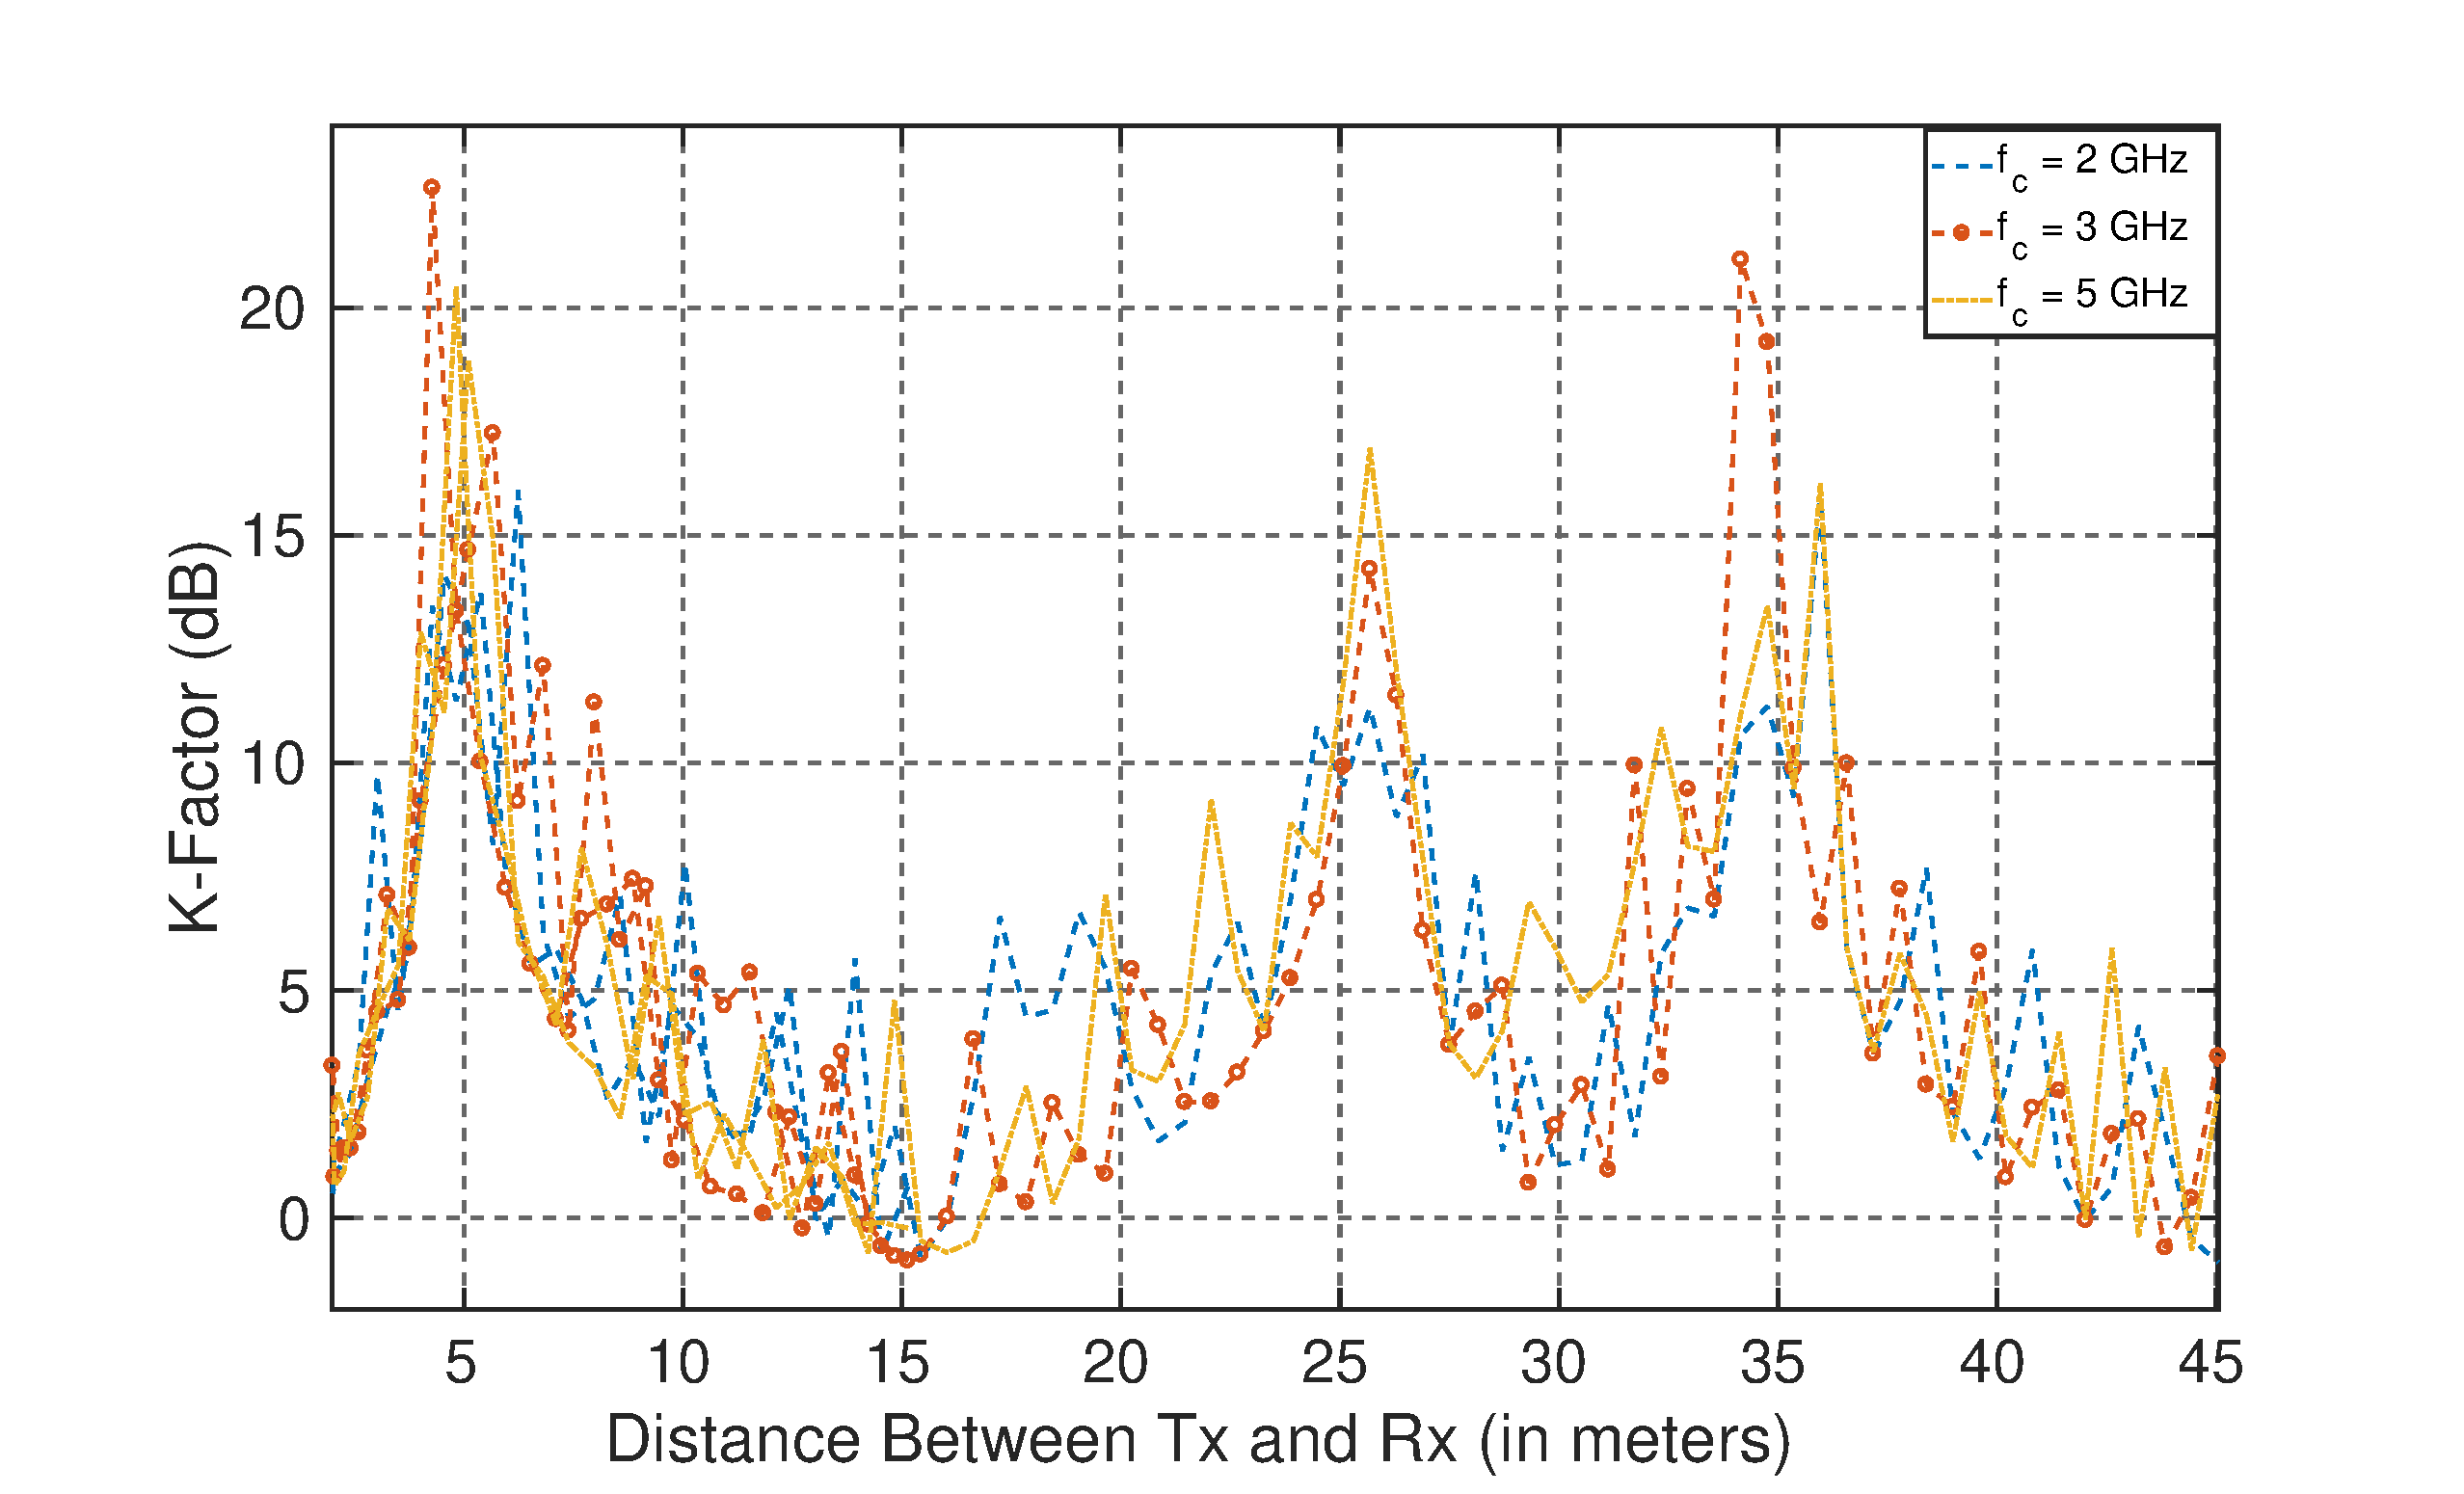
\includegraphics[width=\textwidth,keepaspectratio,height=8cm]{images/Gill/lte_figs/kfactordist.eps} 
\caption{K-factor versus $D_{LOS}$ for different center frequencies $f_c$ = 2, 3 and 5 GHz.}
\end{figure}

\subsection{BER Performance}
To show the impact of varying K-factor on the channel, we computed the BER curve for different modulation schemes of LTE-R with different K-factors. Fig.~\ref{fig:qpsk} shows the BER versus SNR performance for QPSK modulation for different K-factors of the tunnel channel model. The figure clearly demonstrates for higher K-factor we have a better performance while performance degrades as K-factor goes low. Fig.\ref{fig:qam16} shows the $E_b/N_0$ versus BER for 16-QAM and as we can see the BER is higher compared to QPSK. Fig.~\ref{fig:qam64} shows the $E_b/N_0$ versus BER for 64-QAM for different K-factors. And finally we compare all the modulation schemes for the best and worst K-factor in Fig.~\ref{fig:qamall}.

\begin{figure*}[t!]
  \begin{center}
  \subfloat[OFDM-QPSK]
  {\label{fig:qpsk}
  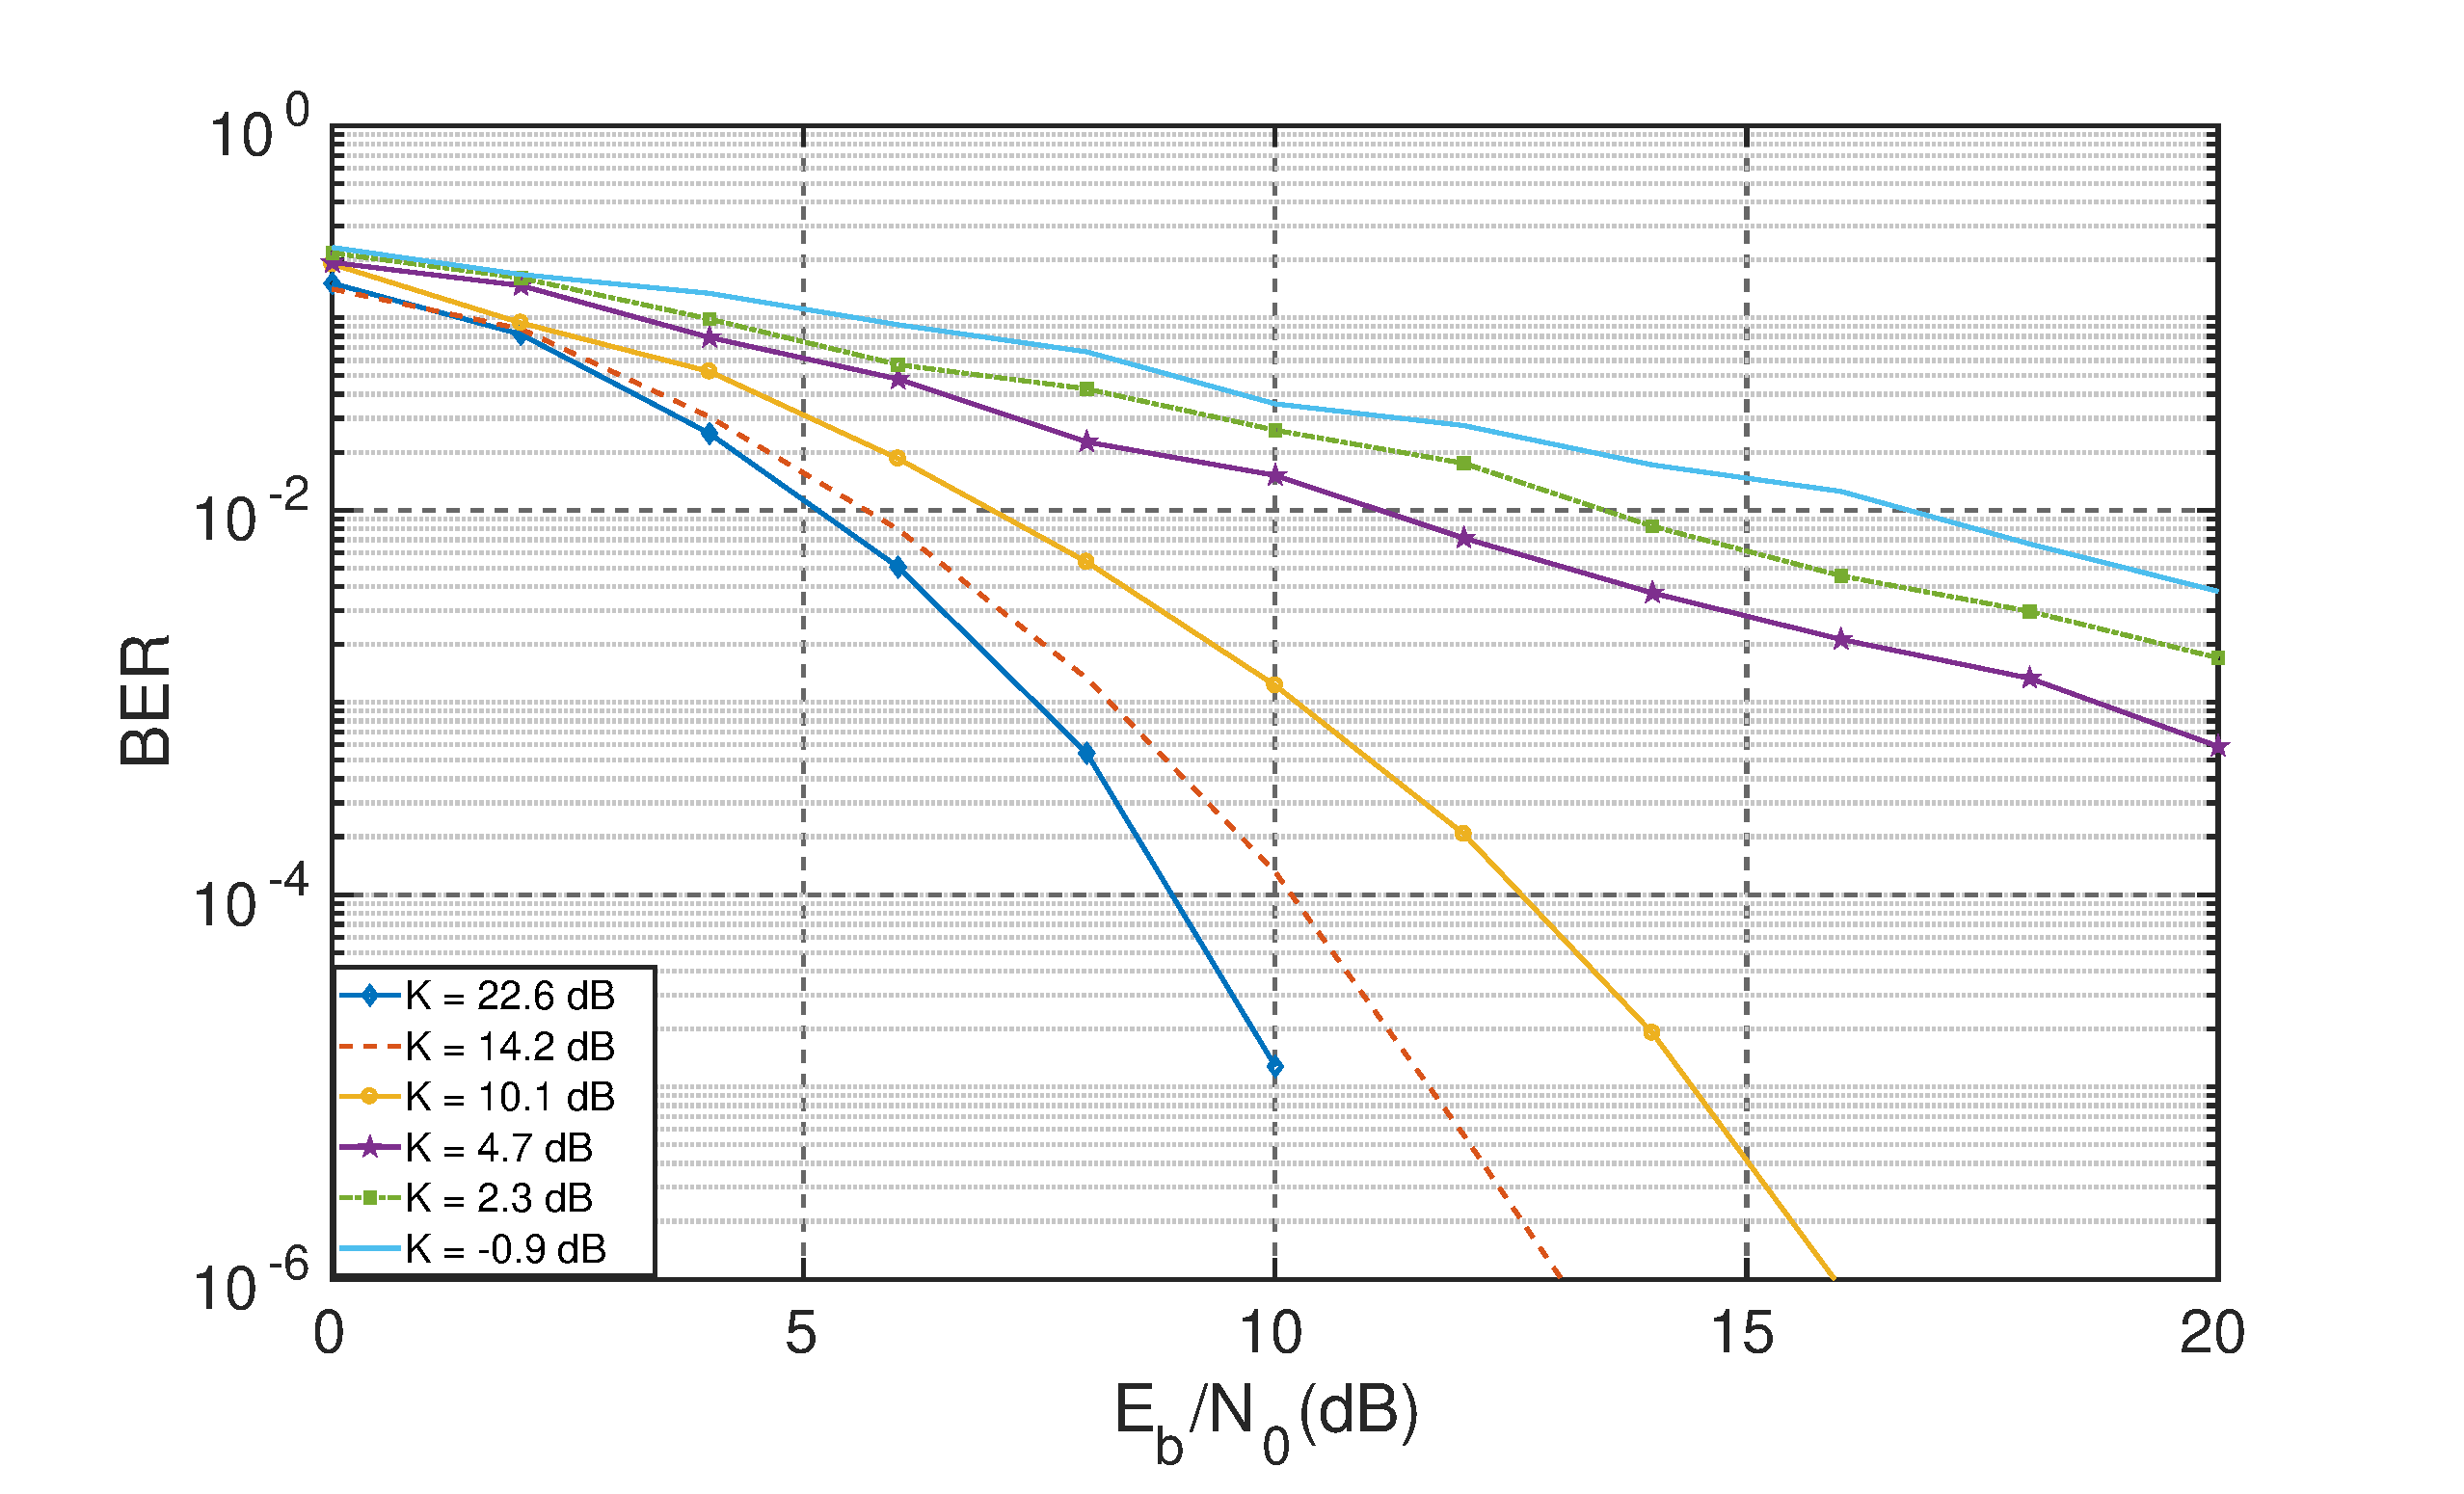
\includegraphics[width=0.46\textwidth]{images/Gill/lte_figs/qpskricean.eps}
  }\hspace{1mm}
   \subfloat[OFDM-16QAM]{\label{fig:qam16}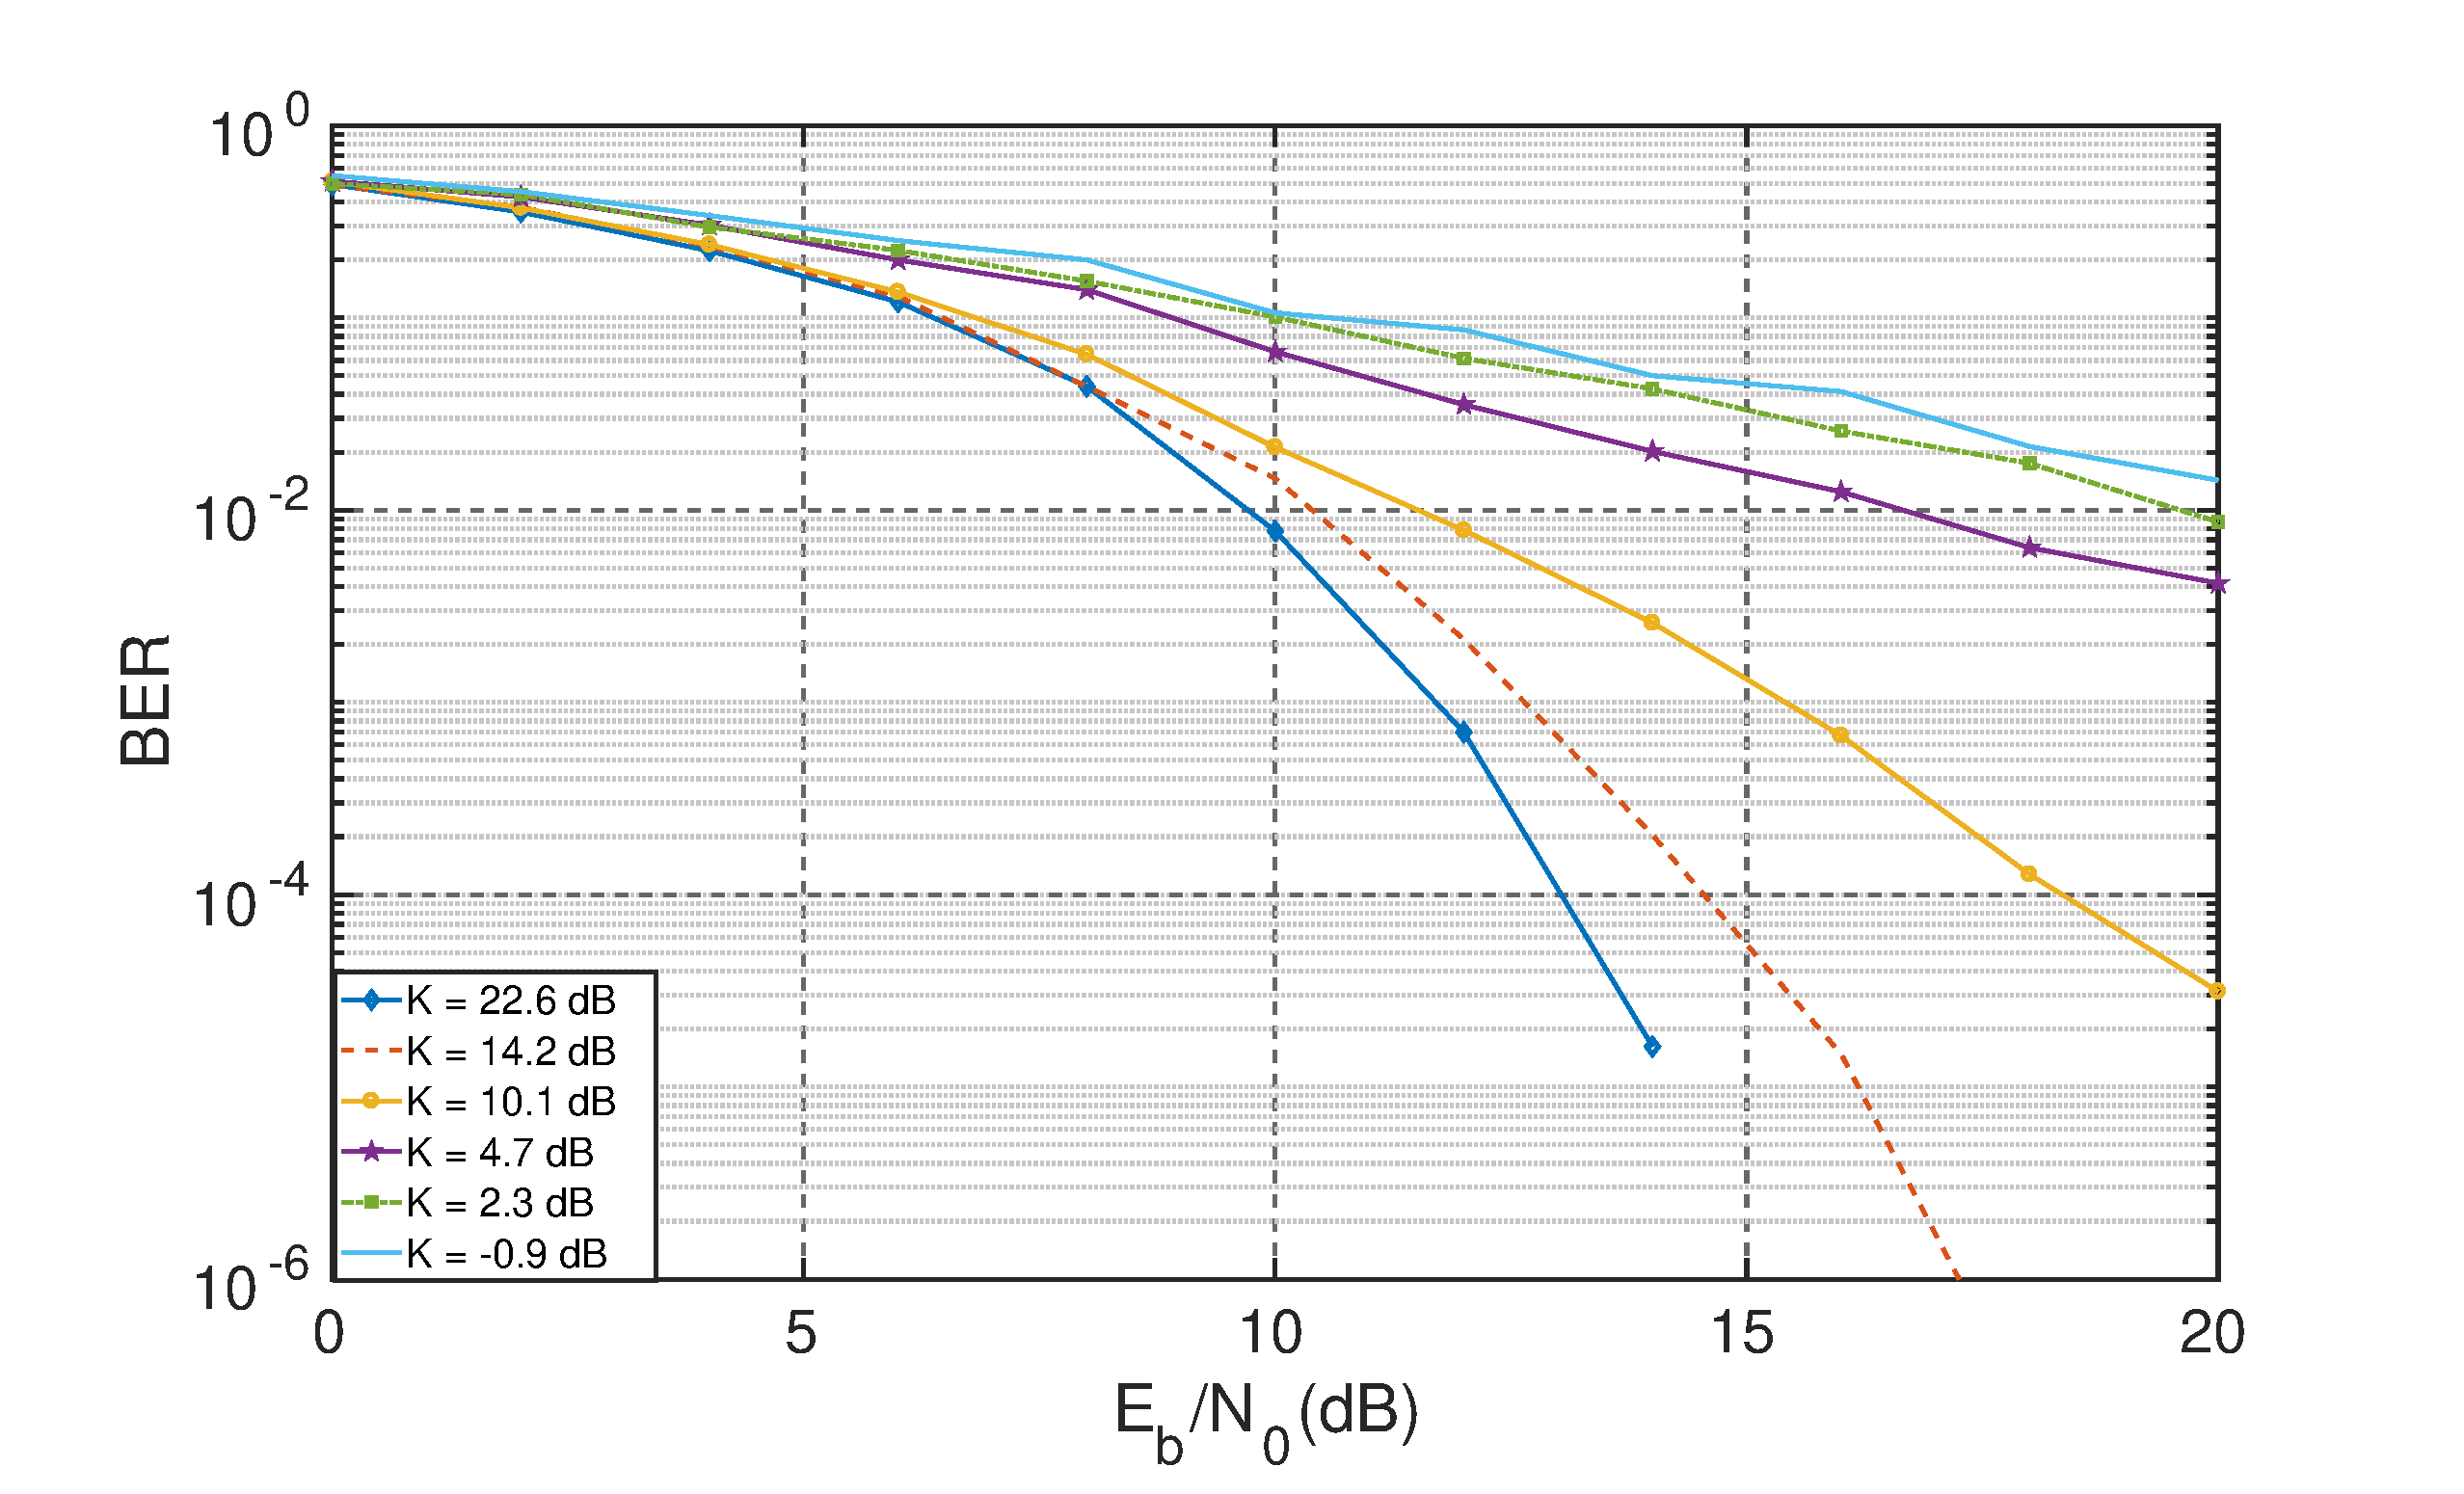
\includegraphics[width=0.46\textwidth]{images/Gill/lte_figs/16qamricean.eps}}\hspace{1mm}
  \subfloat[OFDM-64QAM]{\label{fig:qam64}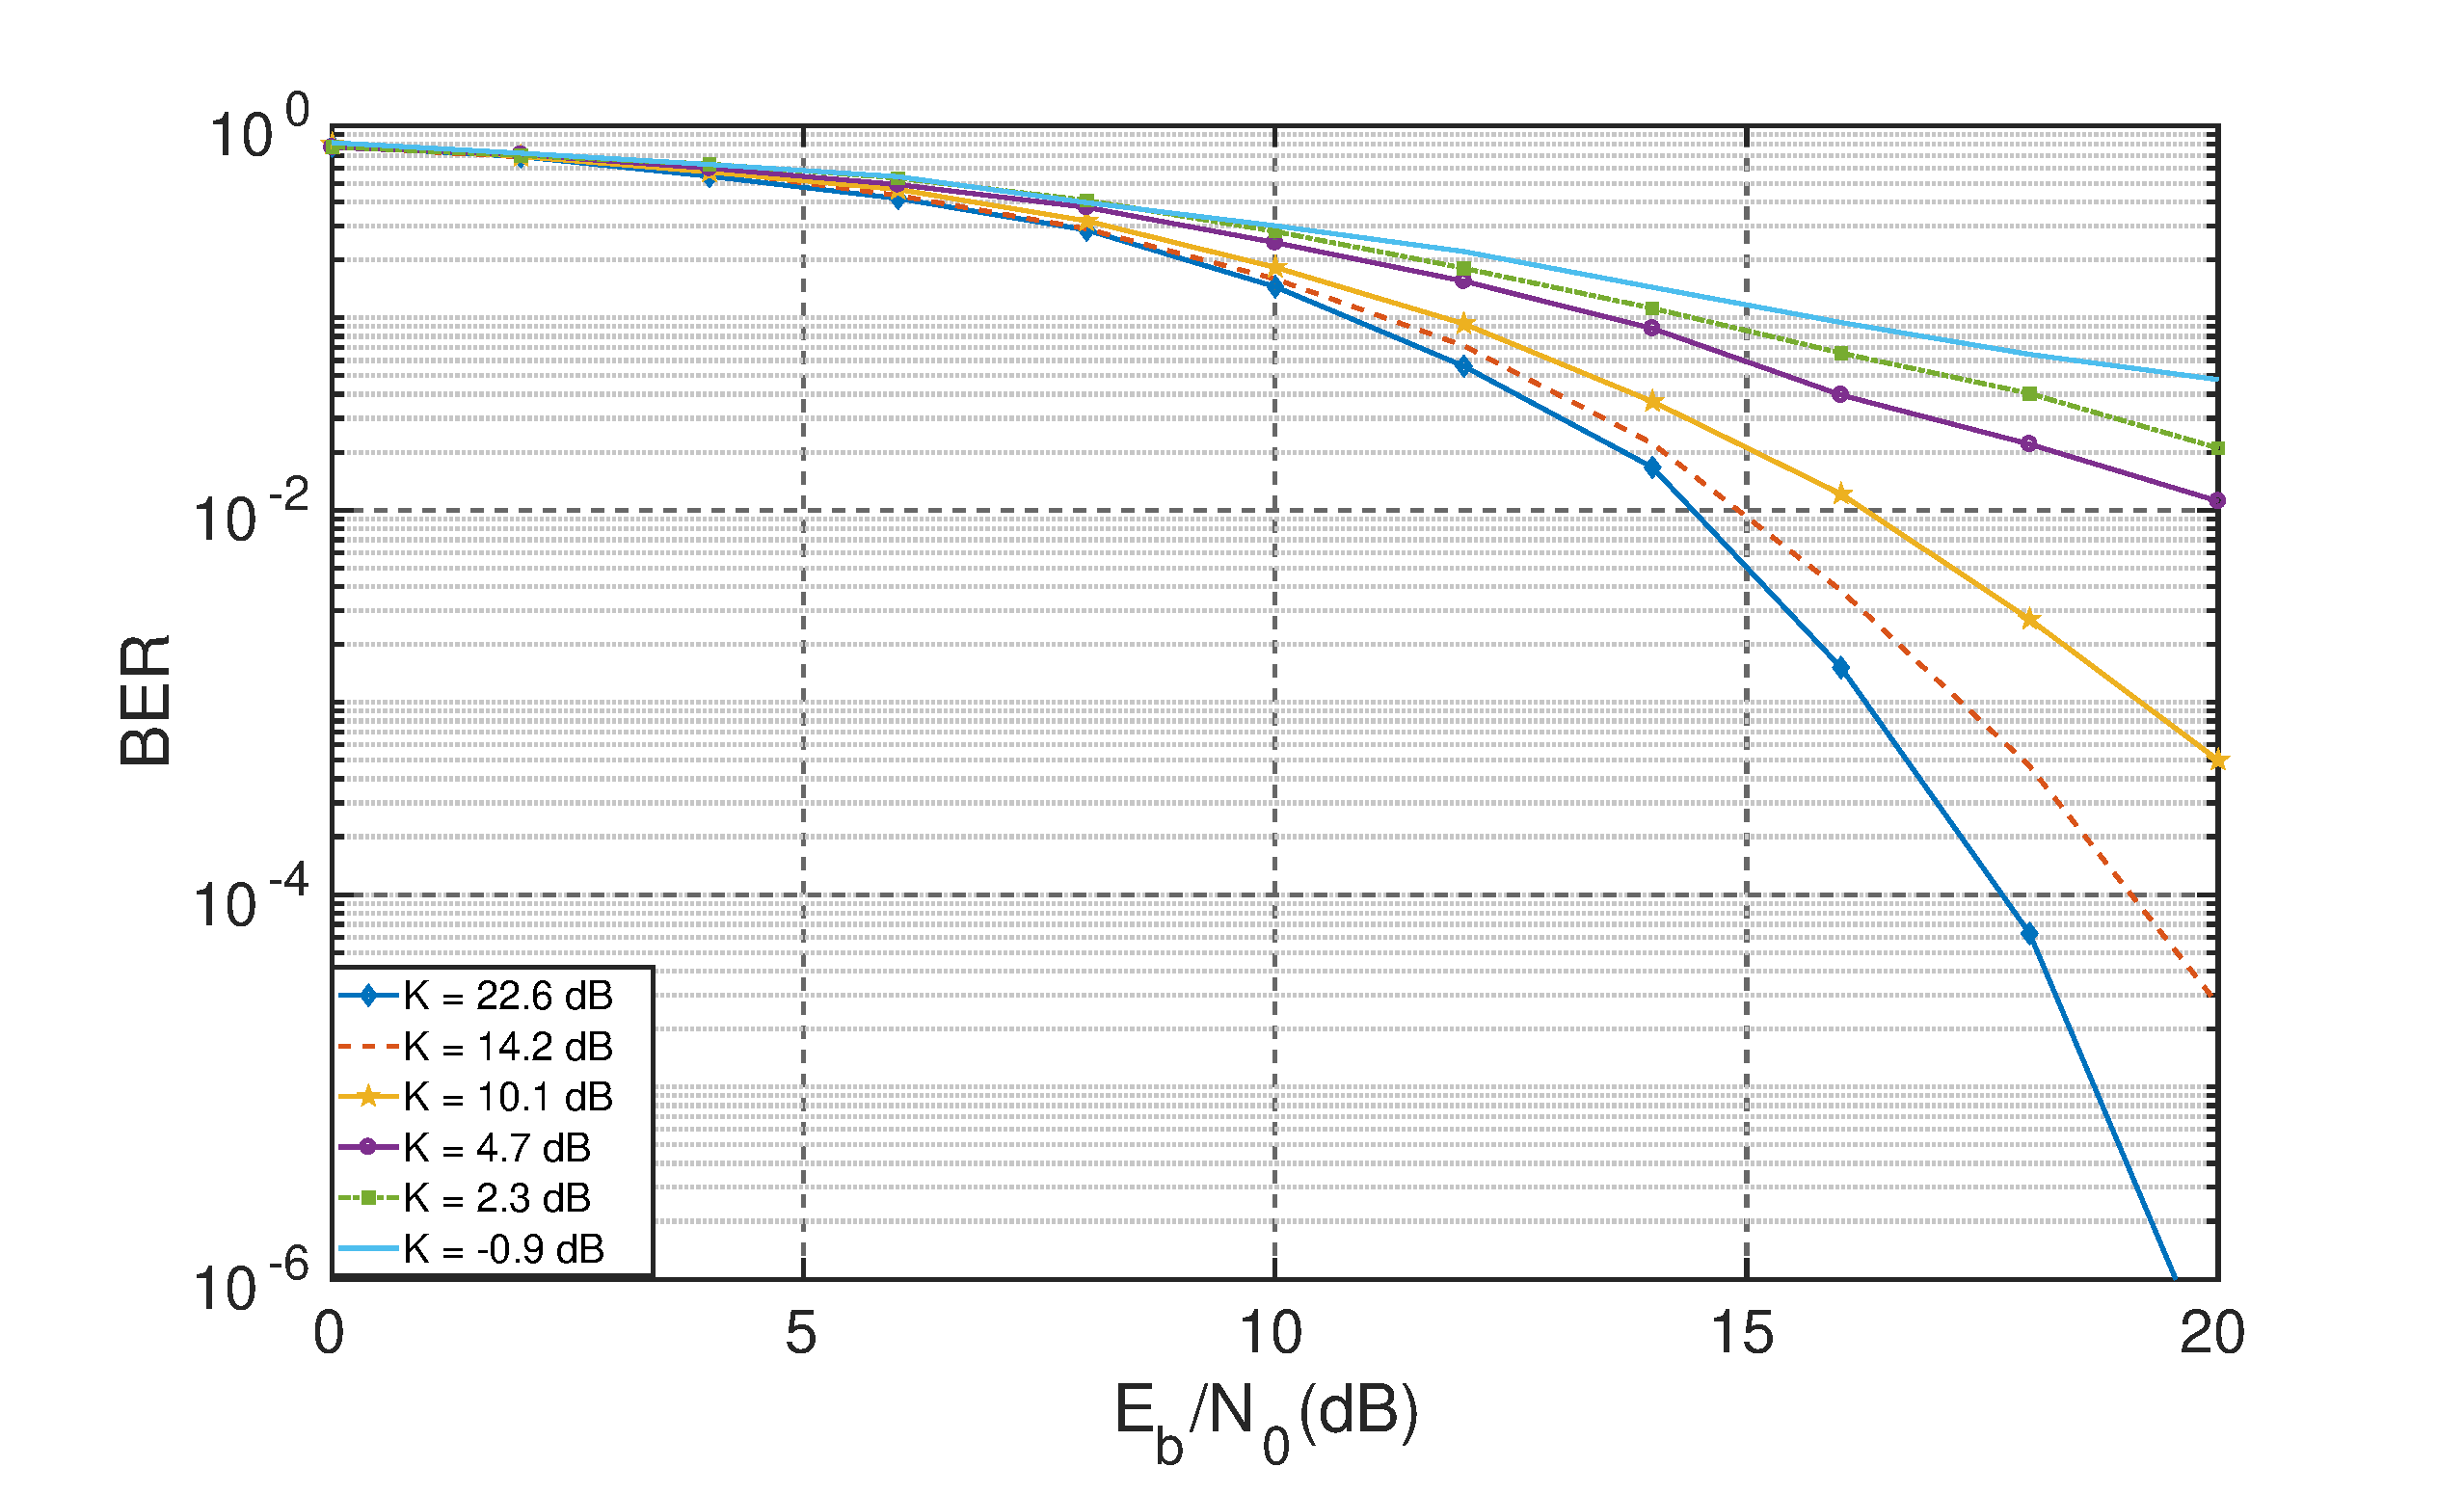
\includegraphics[width=0.46\textwidth]{images/Gill/lte_figs/64qamricean.eps}}\hspace{1mm}
   \subfloat[OFDM-MQAM]{\label{fig:qamall}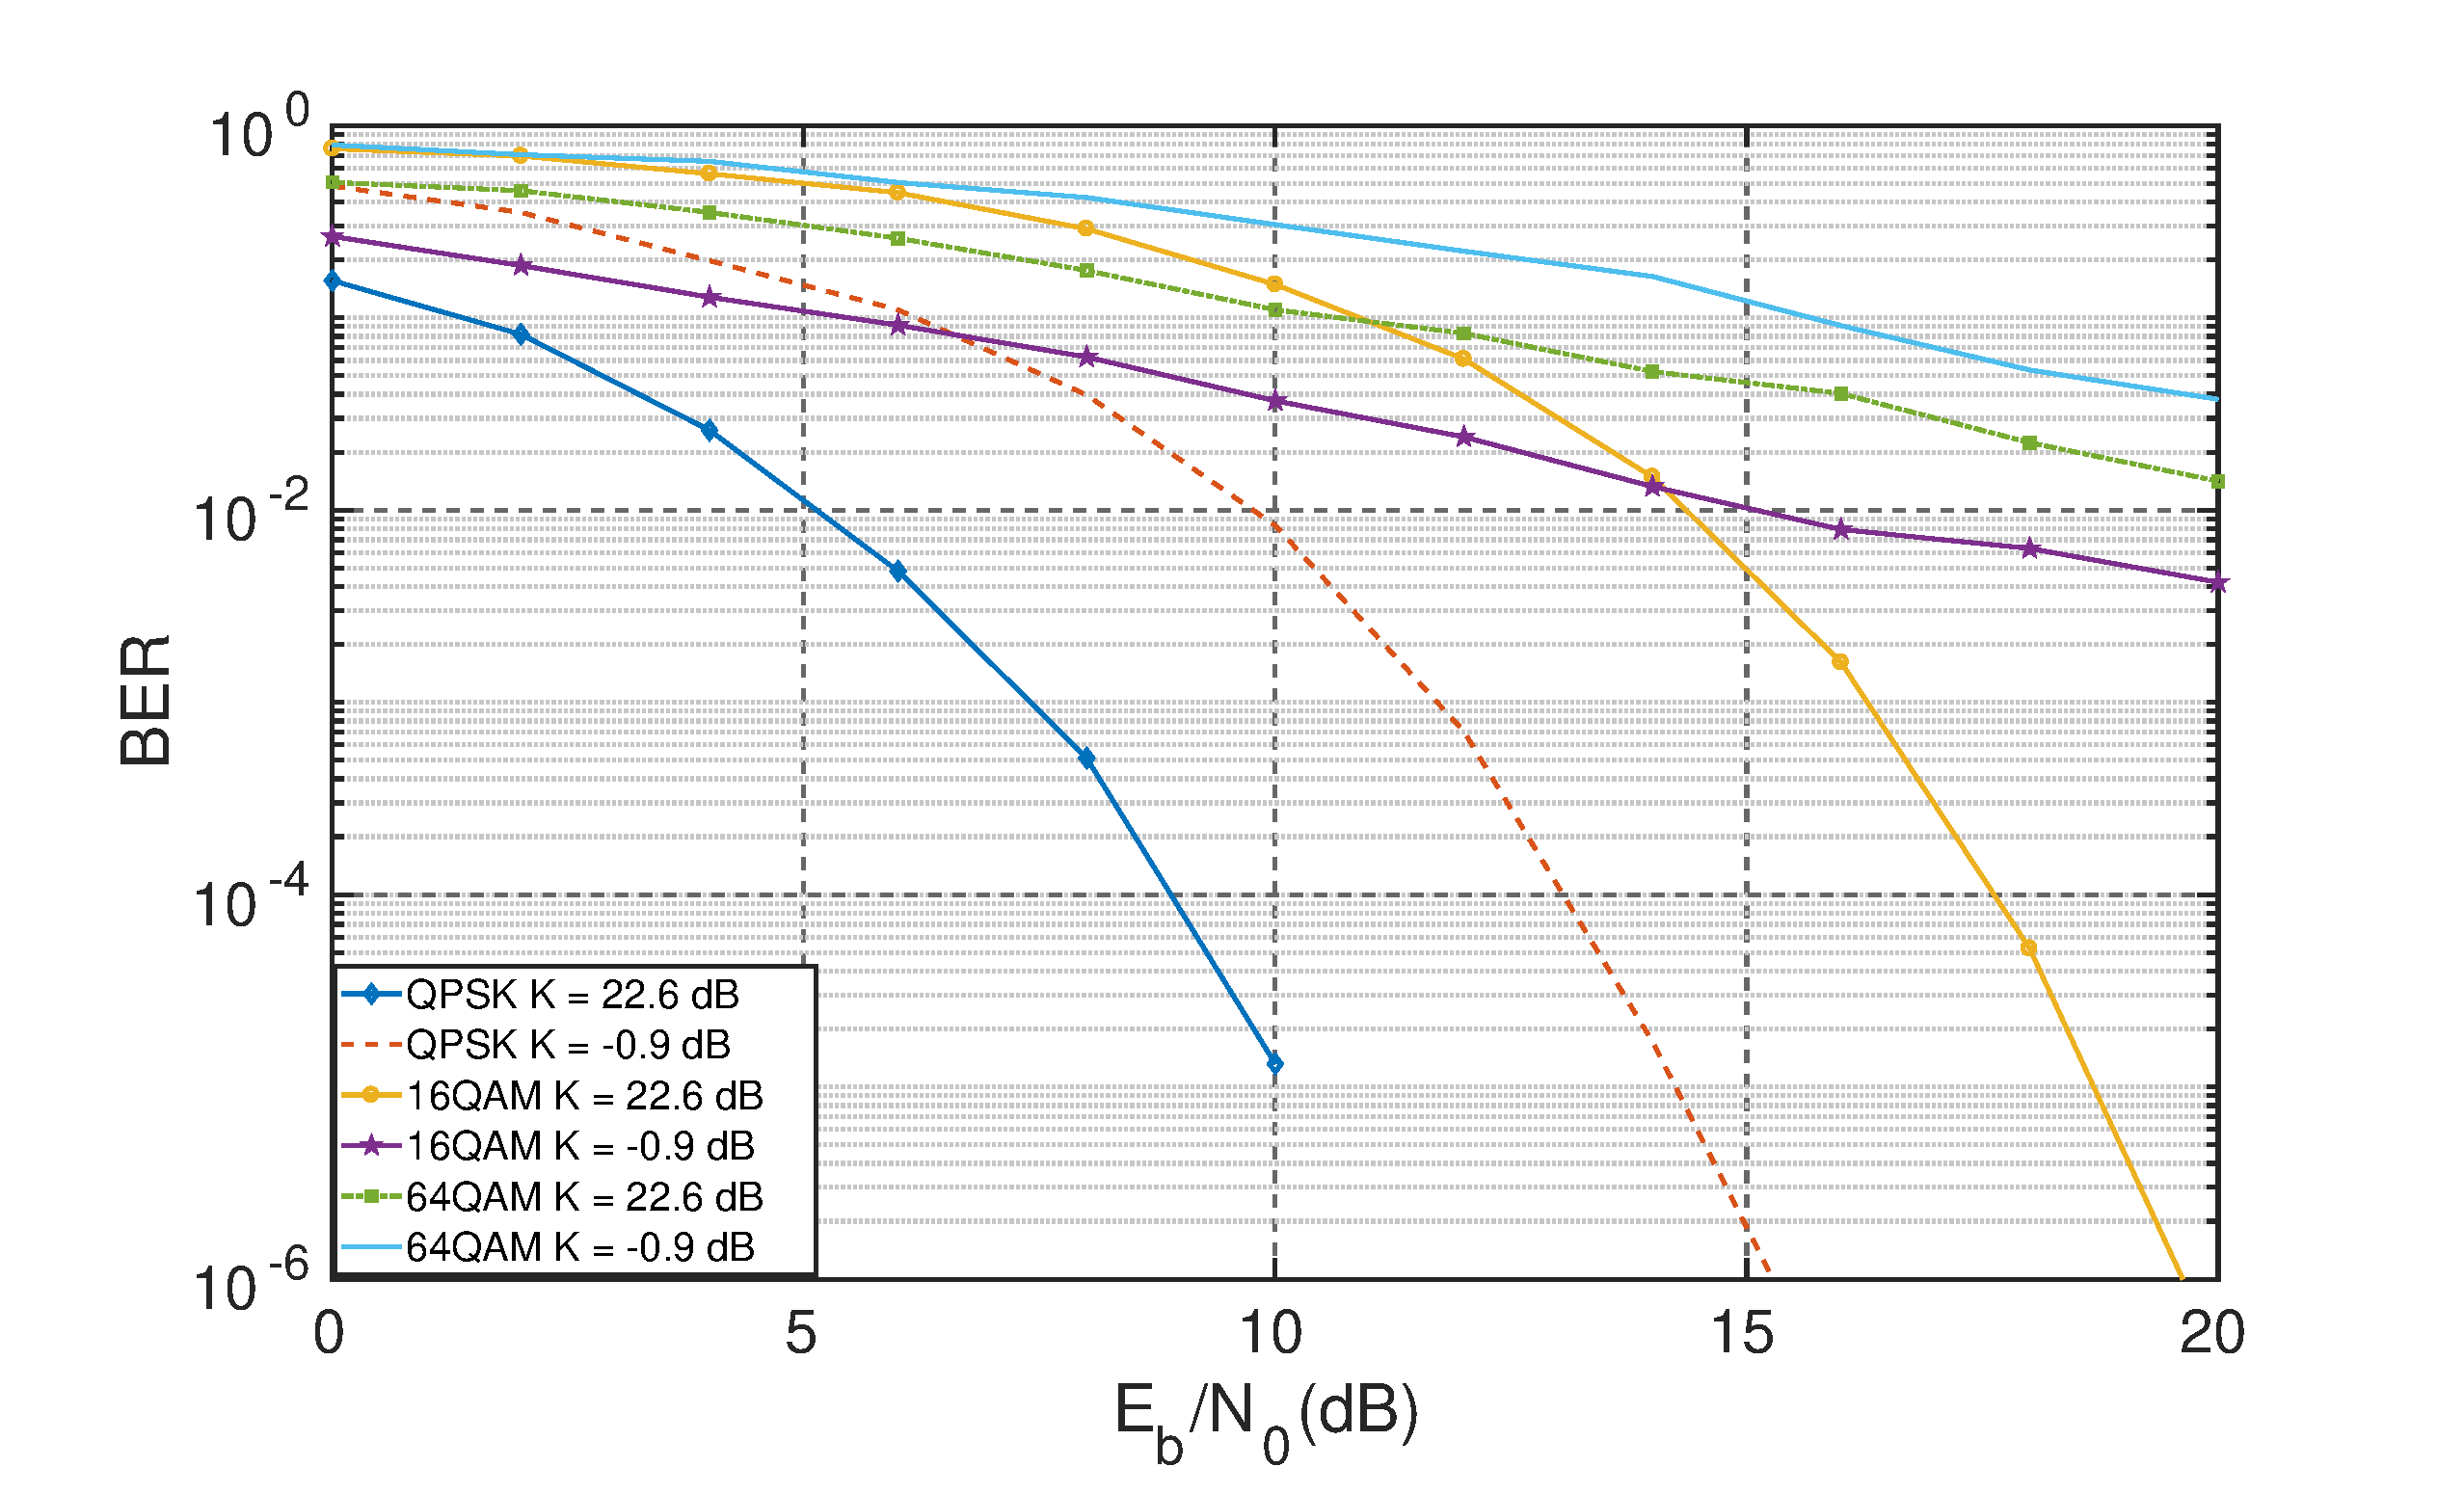
\includegraphics[width=0.46\textwidth]{images/Gill/lte_figs/mqamricean.eps}}\hspace{1mm}
     \caption{Comparison of $E_b/N_0$ verus BER for LTE-R OFDM modulation with different $K$-factors. The first three sub-figures shows the $E_b/N_0$ versus BER for individual modulation schemes employed in LTE-R and in last plot we compare all the modulation schemes for different $K$-factors.} 
\label{fig:modulation}      
   \end{center}
\end{figure*}

In Fig.~\ref{kfactorber} we calculate the BER performance for a high speed train in discrete time-steps. As the train moves towards
the LCX slot the SNR goes high and the SNR decreases as the train moves away. This trend can be seen in the plot, as we move towards the slot the BER curve decreases and it starts increases once we move. It is important to consider here that due to the varying nature of K-factor the BER curve also varies significantly. Hence, by considering the time-varying nature of K-factor we can have a better performance analysis.

\begin{figure}[!ht]
\label{kfactorber}
\centering
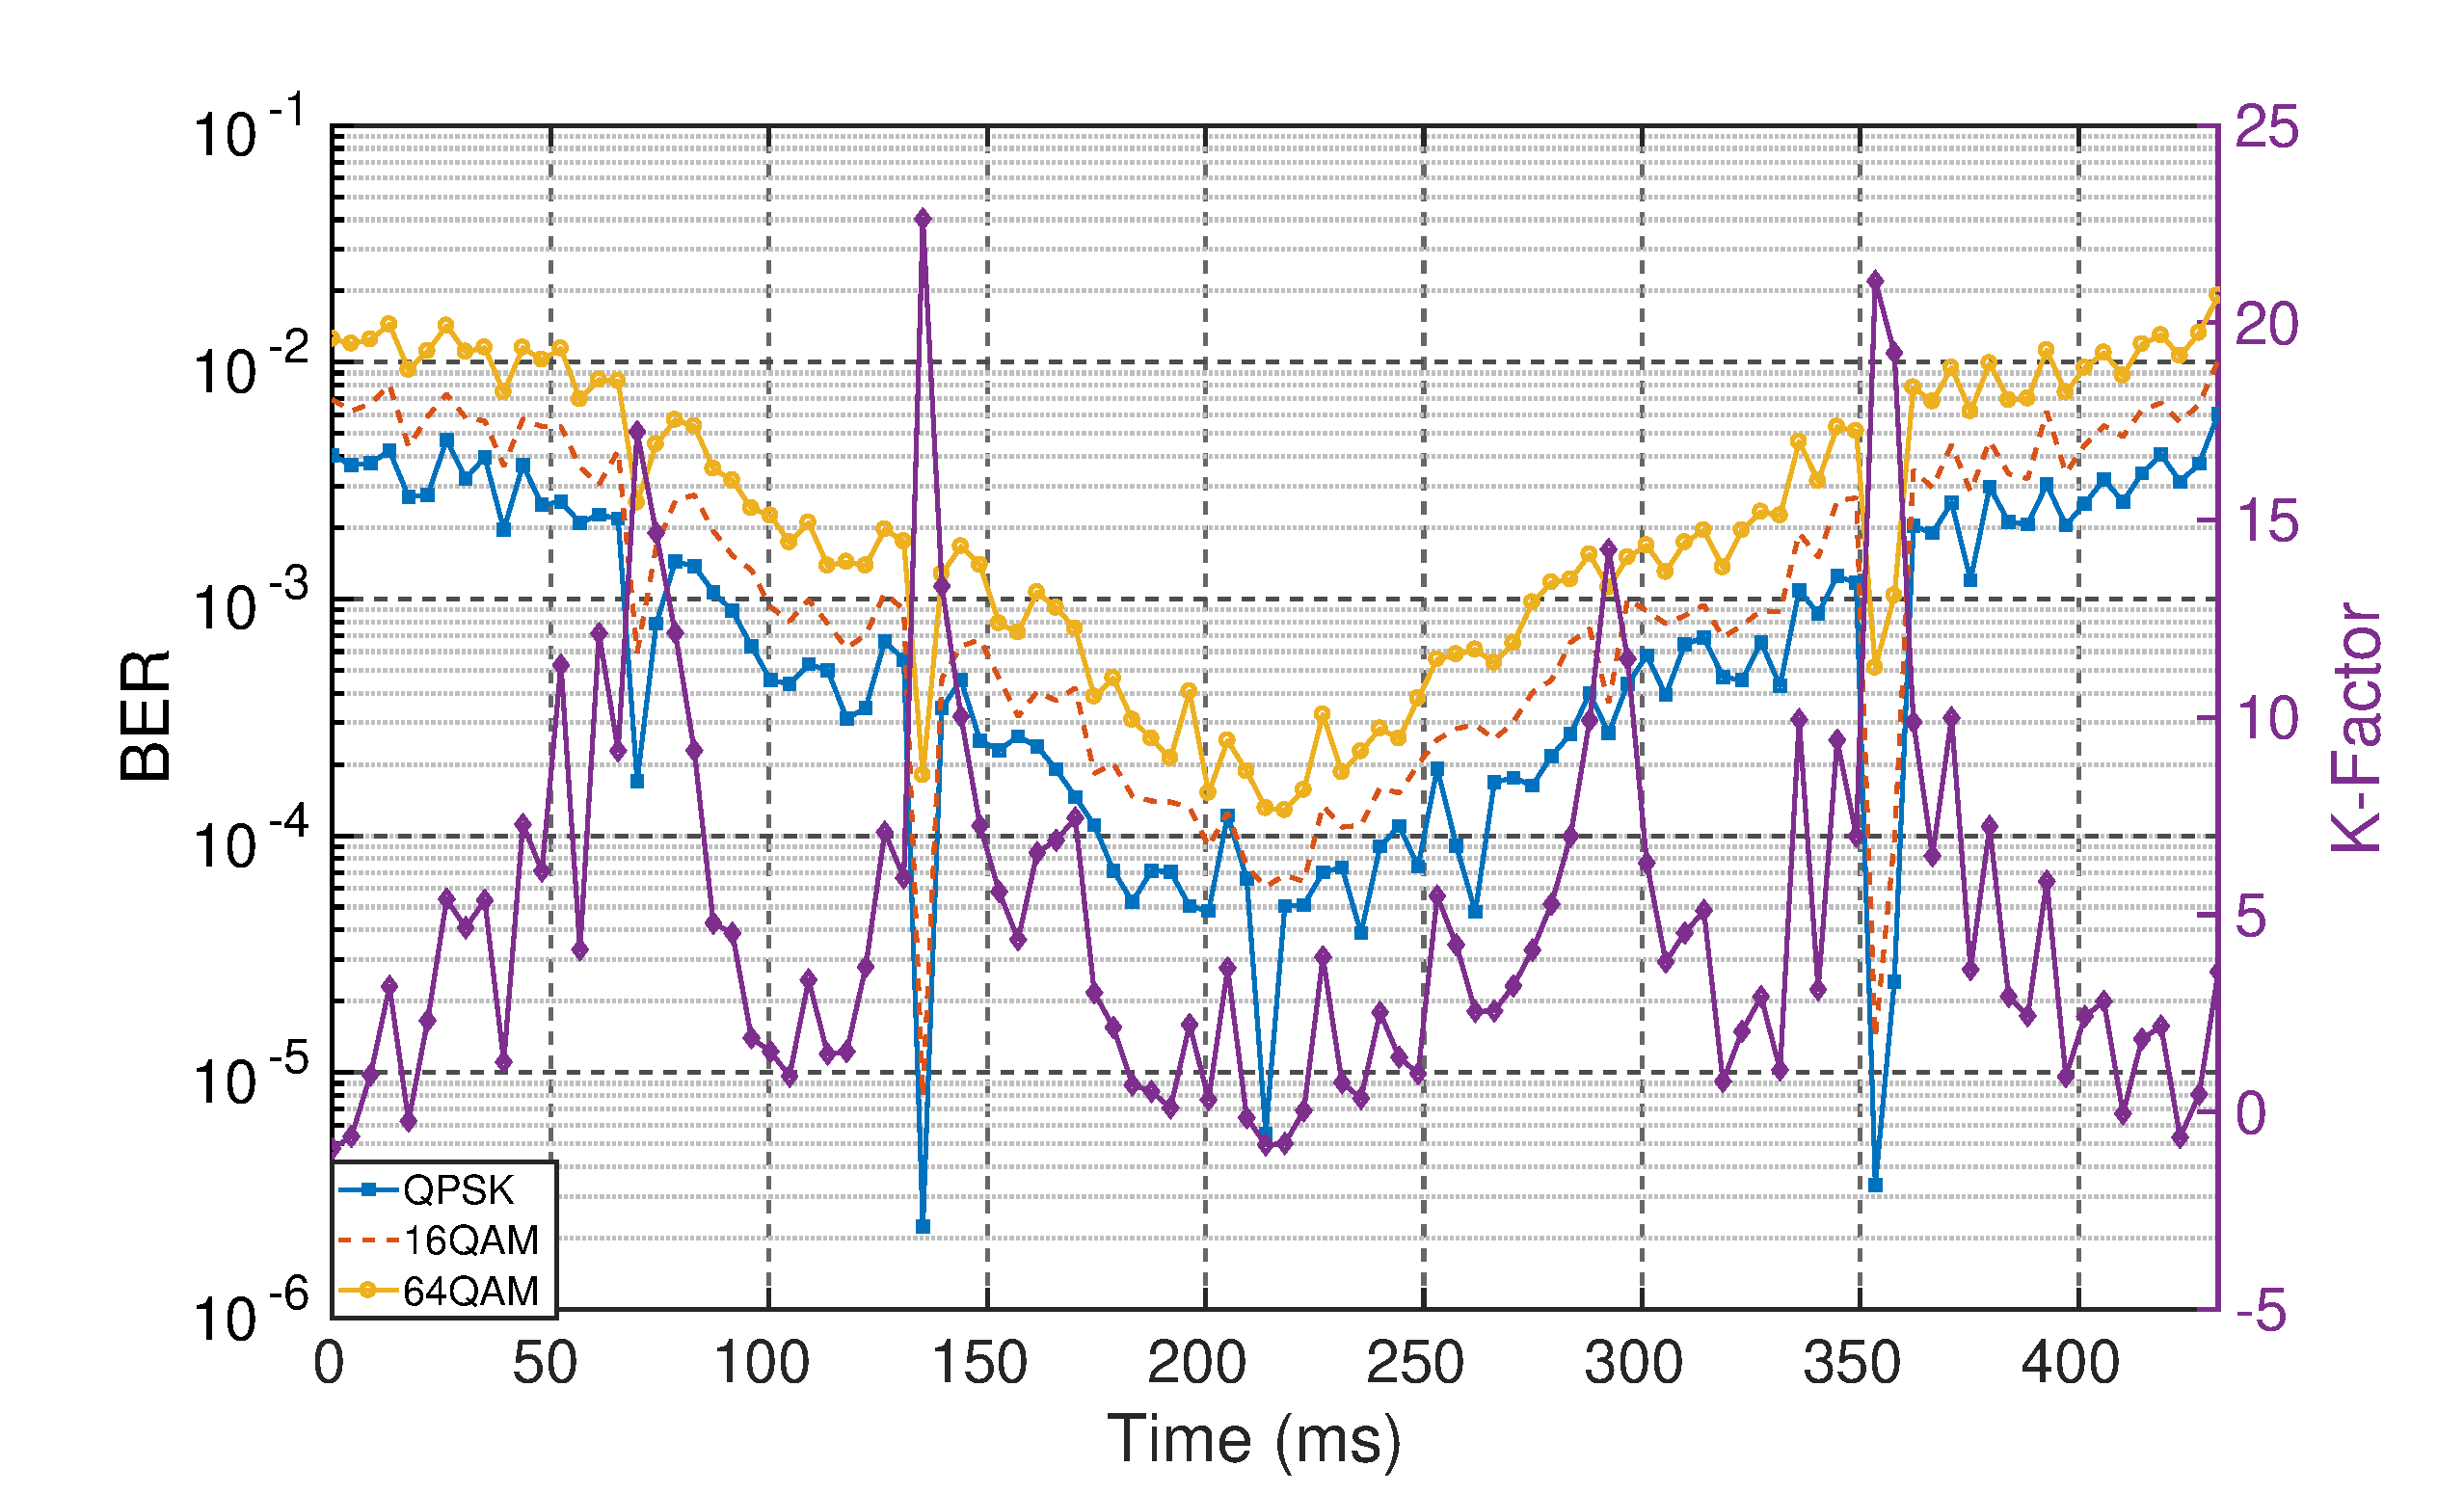
\includegraphics[width=\textwidth,keepaspectratio]{images/Gill/lte_figs/kfactorcontinuous.eps} 
\caption{BER variation with time for HST with different modulation schemes of LTE-R. As the train moves towards
the antenna the general trend of BER goes down with small-scale fluctuations due to varying K-factor.}
\end{figure}

\section{Summary}
We analyzed the BER performance of a LTE-R system for high speed trains inside tunnel environments using our proposed channel model. For the implementation
of our channel, we first derived the time-series K-factor function using the classical two-ray propagation model. We then analyzed the LTE-R performance under our channel model for different modulation schemes for various K-factors. Finally, we compared all the modulation schemes under worst and best K-factor, and we observed that for low $E_b/N_0$
sub-carriers must be modulated with QPSK for maintaining reliable communication link.



